\documentclass[12pt, a4paper, titlepage]{extreport} 
\usepackage[top=2cm]{geometry}
\usepackage{csquotes}
\usepackage[utf8]{inputenc} 
\usepackage{amssymb, amsmath, mathrsfs, amsthm,amscd} 
\usepackage[russian]{babel} 
\usepackage[footnotesize]{caption2} 
\usepackage{indentfirst} 
\usepackage{graphics, graphicx} 
\usepackage[noend]{algorithmic} 
\DeclareGraphicsExtensions{.pdf,.png,.jpg} 
\usepackage{wrapfig} 
\usepackage{listings}
\usepackage{color}
\usepackage{amsmath}
\usepackage{enumitem}





\begin{document} 
	\begin{titlepage} 
		\begin{center} 
			
			
\includegraphics[width=55mm]{msu} 
			\line(1,0){400}
			
			Московский государственный университет имени М.В.~Ломоносова\\ 
			Факультет вычислительной математики и кибернетики\\ 
			Магистерская программа «Большие данные: инфраструктуры и методы решения задач»
			
			\vspace{3.5cm} 
			
			{\Large Магистерская диссертация}
			
			\vspace{1cm} 
						
			{\Large{\textbf{Автоматическое удаление физиологических артефактов в данных электроэнцефалограммы (ЭЭГ)\\}}}
			
			\vspace{0.7cm} 
			
			
		\end{center} 
		
		\vfill 

		\begin{flushright} 
			Работу выполнил\\
			\textbf{Студент}\\ 
			Китов Иван Денисович
		\end{flushright}

%		\vspace{0.1cm}
				
		\begin{flushright} 
			\textbf{Научный руководитель}\\ 
			к.т.н. \\ Ступников Сергей Александрович\\
			\textbf{Консультант:}\\
			м.н.с ФИЦ ИУ РАН\\ Шанин Иван Андреевич 
		\end{flushright} 
		
		\vfill 
		
		\begin{center} 
			Москва, 2020 
		\end{center} 
		
		\enlargethispage{4\baselineskip} 
		
	\end{titlepage}

		
%	\newpage
	\setcounter{page}{2}
	\tableofcontents
	
	\chapter*{Введение}
	\addcontentsline{toc}{chapter}{Введение}
	В настоящее время существует множество методов медицинских исследований организма человека: начиная с обычного измерения пульса, заканчивая магнитно резонансной томограммой. В частности, за последние 50 лет совершен значительный прогресс в исследовании мозга, в частности с помощью электроэнцефалограммы \cite{6}. Этот метод стал широко доступен по всему миру благодаря своей возможной дешевизне и нетребовательности к оборудованию. Если сравнивать, например, с магнитно-резонансной томографией (МРТ), то оборудование, необходимое для проведения этого исследования, имеется в куда меньшем количестве больниц, чем для ЭЭГ \cite{37}. К тому же, ЭЭГ позволяет проводить исследование во время выполнения каких-либо действий, то есть не ограничено состоянием покоя (resting state). Аналогично, оборудование для проведения ЭЭГ обычно стоит гораздо дешевле и имеет множество вариаций: от 4 до 128 электродов в шапочке. Конечно, с увеличением количества электродов и вариаций (беспроводная опция), увеличивается и цена, которая может достигать 10-15 тысяч долларов, как, например, ABM B-Alert X10 EEG \cite{38}. Однако, следует дополнительно отметить, что пусть ЭЭГ и является достаточно эффективным методом исследования мозга, он всё ещё не настолько эффективен, как инвазивные методы \cite{39}. Но преимущество в виде неинвазивности зачастую перекрывает все недостатки.
	\\ Электроэнцефалография (ЭЭГ) – высокоинформативный метод диагностики состояния нервной системы, основанный на регистрации биоэлектрических потенциалов коры головного мозга (ГМ) в процессе его жизнедеятельности.
	Результатом ЭЭГ является электроэнцефалограмма — графическая запись ритмов мозга в виде кривых линий.\\
 	В то же время, расшифровка данных и очистка их от артефактов зачастую проводится без использований средств автоматизации - с помощью экспертов. В медицинских исследованиях фрагменты ЭЭГ, содержащие артефакты, удаляют вручную,что обусловлено высокой степенью моральной и юридической ответственности перед пациентом в случае ошибочной интерпретации данных ЭЭГ. На настоящий момент существует множество методов удаления артефактов различной природы: глазодвигательных, моргания, сокращения мышц итд.  \cite{ 1,2,3,4,5,6,7, 8}. В этой работе предлагается метод, основывающийся на исследовании графовой составляющей сигналов ЭЭГ. \\
 	Очистка ЭЭГ от артефактов является важной задачей в связи с тем, что артефакты зачастую вносят значимые шумы в данные и могут не позволить увидеть какие-либо важные патологии мозга\\
 	Естественной выглядит идея применить нейросети для выявления артефактов, т.к. они показали свою эффективность в работе с наборами данных, у которых много признаков и зависимости часто являются неочевидными для человека и классических методов машинного обучения. Таким образом, эта работа посвящена:
 	\begin{enumerate}
 		\item Обзору и анализу современных методов выявления артефактов в ЭЭГ
 		\item Разработке собственного подхода, основанного на исследовании структуры активации электродов с помощью машинного обучения и построения модели для выявления различных артефактов
 		\item Реализации метода, способного работать с произвольными данными ЭЭГ, который легко реплицируется и применим на широком классе данных
 	\end{enumerate}
 	
	\chapter*{Постановка задачи}
	\addcontentsline{toc}{chapter}{Постановка задачи}
	Целью данной магистерской диссертации является разработка универсального метода, позволяющего выявить артефакты в ЭЭГ.\\
	Для достижения поставленной цели, необходимо выполнить следующие шаги:
	\begin{enumerate}
		\item Исследовать существующие методы выявления артефактов
		\item Предложить собственный метод выявления артефактов, который может быть масштабирован и применим к произвольным данным
		\item Реализовать предложенный метод и оценить его эффективность
		\item Применить его для устранения артефактов на произвольных наборах данных, чтобы валидировать работоспособность.
	\end{enumerate}
	\chapter*{Обзор известных методов и средств решения задачи}
	\addcontentsline{toc}{chapter}{Обзор известных методов и средств решения задачи}
	\section*{Общая информация про ЭЭГ: способы проведения исследования, типичные схемы}
	\addcontentsline{toc}{section}{Общая информация про ЭЭГ: способы проведения исследования, типичные схемы}
	\subsection*{Биологическая основа ЭЭГ}
	ЭЭГ основано на том, что, в кортикальной нервной клетке, состоящей на 70-80\% из воды и на 20-30 \% из белка и липидов, и может быть классифицирована на основании ее структуры и функционирования тройки: 
	\begin{enumerate}
		\item сома - клеточное тело,
		\item дендриты - многочисленные короткие импульсы сомы,
		\item Аксон - переносчик сигнала или носитель от сомы к другому нерву или мышечной клетке.
	\end{enumerate}
	 Промежуток между аксоном одной нервной клетки и дендритами другой называется синапсом и нейротрансмиттеры, также называемые химическими передатчиками, отвечают за транспортировку сигнала через него.
	Схема, изображающая кортикальный нейрон, который получает импульсы от нескольких тысяч нейронов, показана ниже\\
	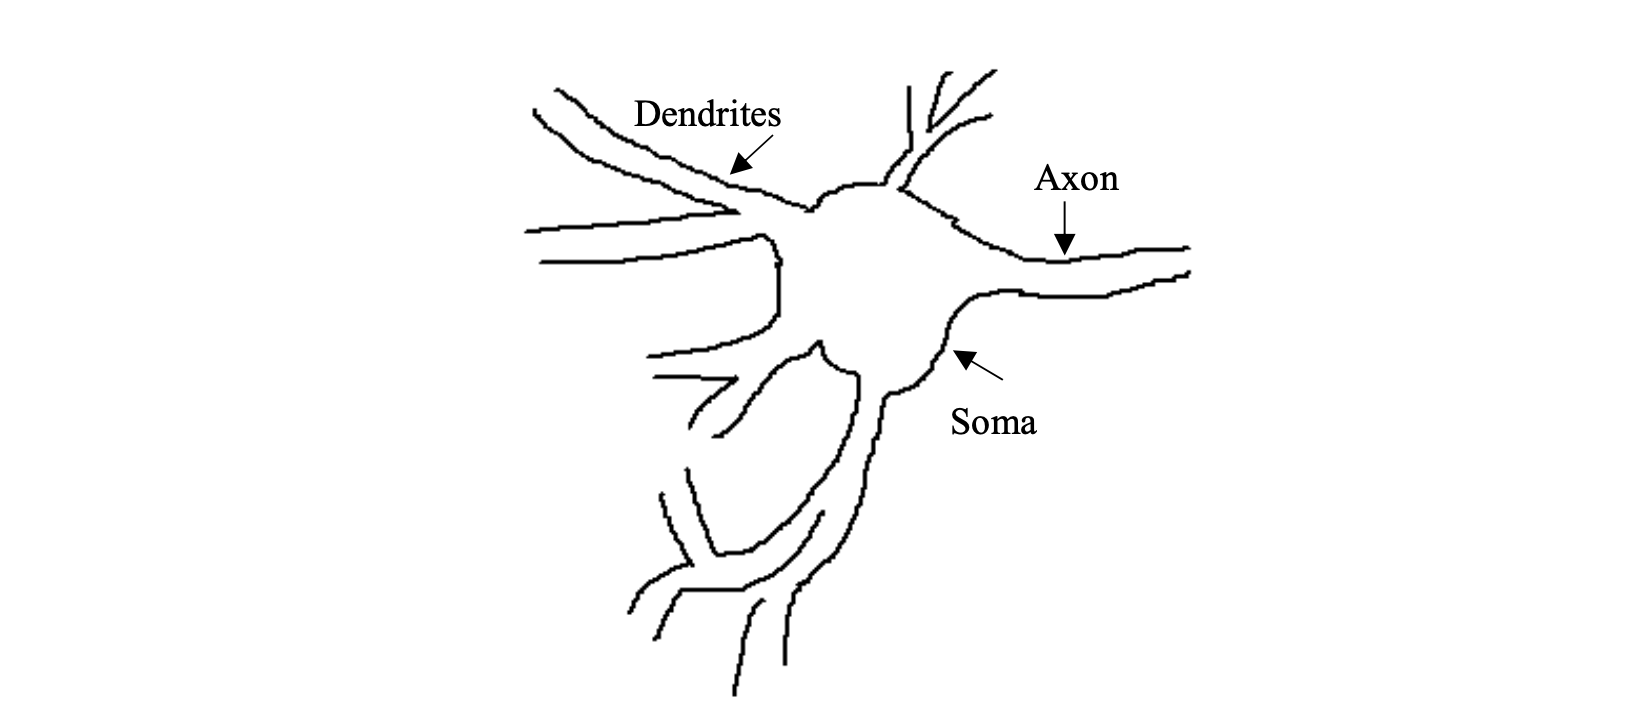
\includegraphics[scale=0.5]{neuron_structure}\\
	Биоэлектричество, генерируемое за счет нервного возбуждения, может быть измерено на коже головы в виде ЭЭГ с использованием влажных или сухих электродов.\cite{41}
	\subsection*{Позиции электродов и схемы расположения}
	Система 10-20 - это международный метод, рекомендованный Международной федерацией клинической нейрофизиологии (International Federation of Clinical Neurophysiology) для описания расположения 21 электрода на коже головы. Он обычно используется для измерения ЭЭГ из четырех основных частей головного мозга: лобной, центральной (сверху), височной (по бокам) и затылочной (сзади). Электроды равномерно распределены в зависимости от размера и формы черепа и расположены на расстоянии 10\% и 20\% друг от друга. В зависимости от типа применения, ЭЭГ можно извлечь из 8 до 32 каналов. Измерения ЭЭГ могут быть биполярными или униполярными. Первое относится к разности потенциалов между набором электродов, а второе - к потенциалу каждого отдельного электрода по отношению к электроду сравнения.\\
	Система Queen Square (QSS) предпочтительнее системы 10-20 для измерения вызванных потенциалов (Evoked Potentials - EPs), поскольку боковые затылочные отведения расположены дальше от центра, что позволяет улучшить регистрацию распределения по коже головы шаблонных визуальных потенциалов. Если электроды расположены ближе друг к другу, то ток ведущего поля протекает всё сильнее внутри кожи, чем между электродами,
	таким образом, снижается чувствительность электрода. Опорные точки nasion на верхней части носа и inion у основания черепа используются в качестве ориентиров для размещения электродов.\\
	\begin{center}
		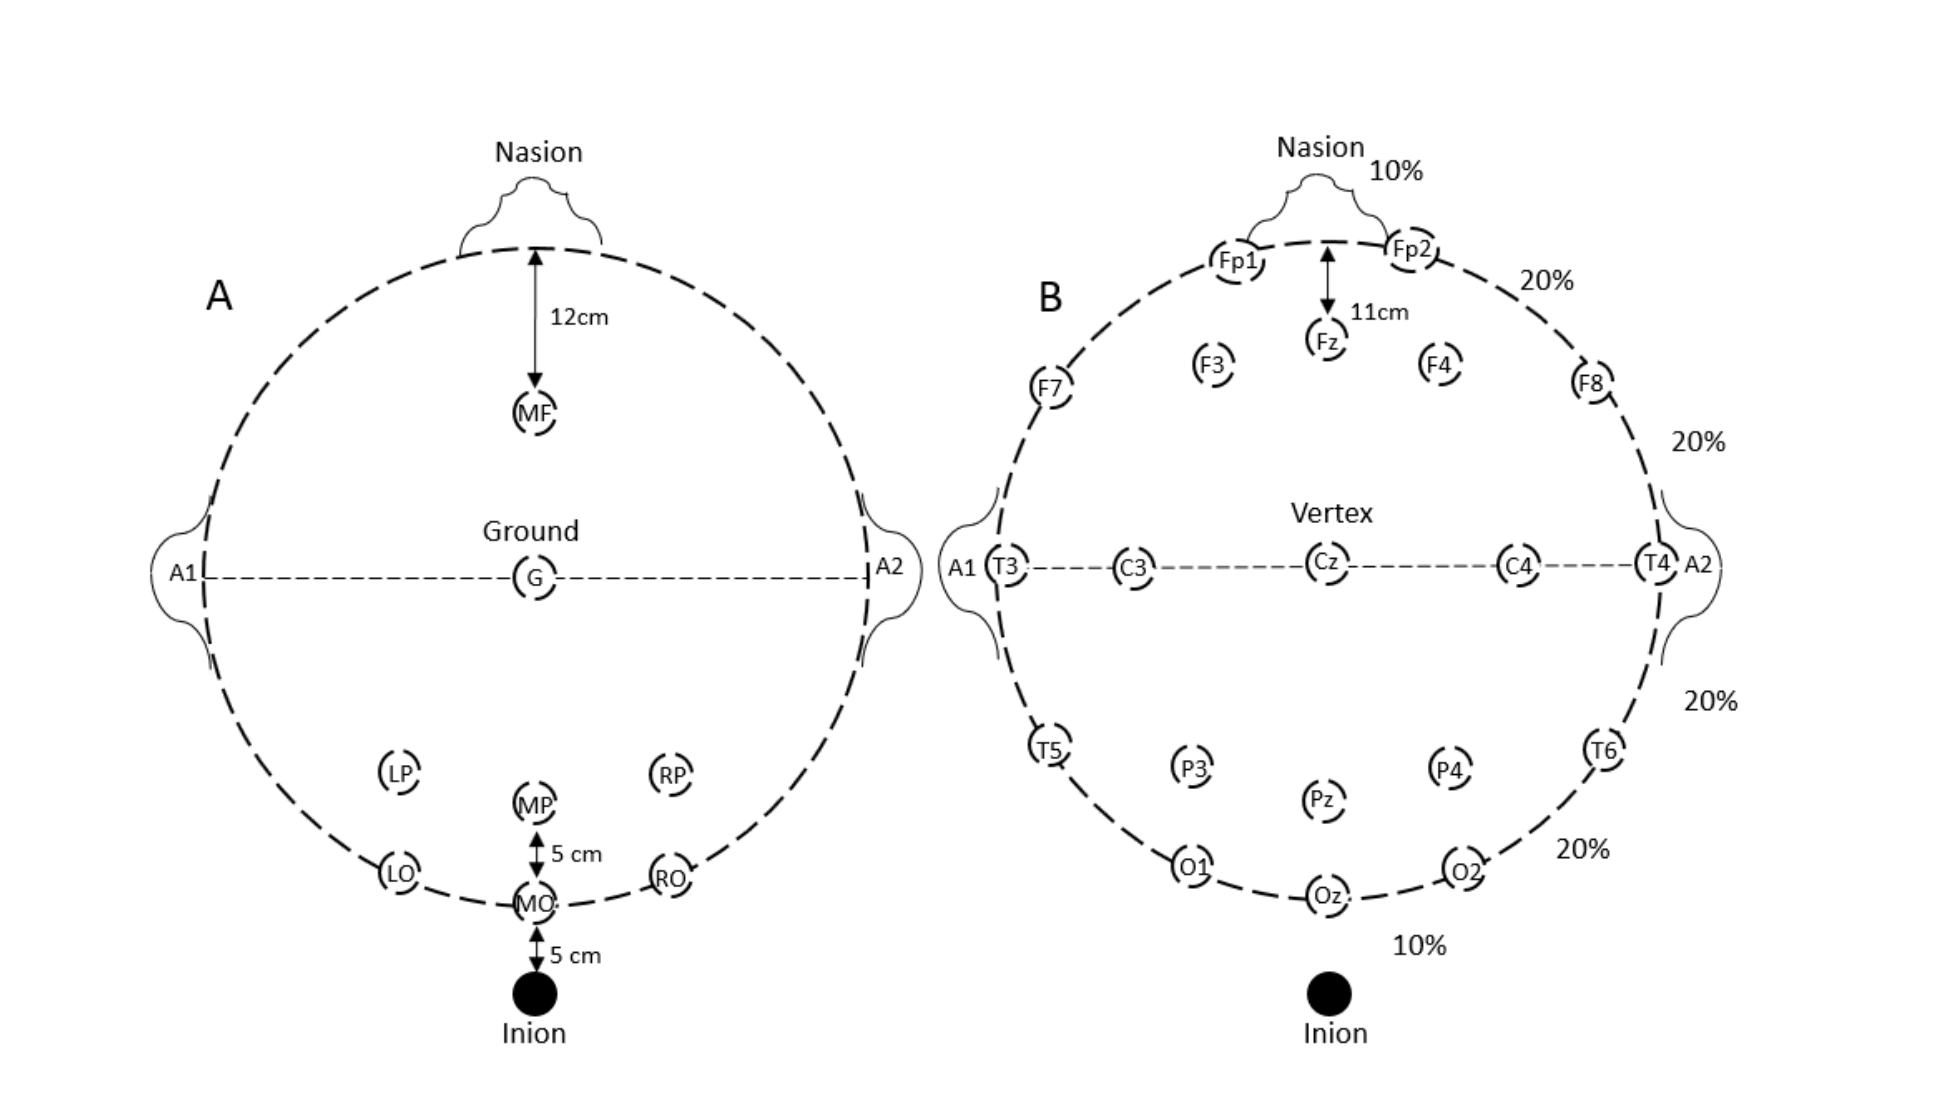
\includegraphics[scale=0.5]{placement_system}\\
		Различия между системами QSS (A) и 10-20 (B)
	\end{center}
	Для EPs, использующих QSS, должно быть записано не менее четырех каналов. Как в 10-20, так и в QSS четные и нечетные номера электродов относятся к правой и левой стороне головы соответственно. G (в системе QSS) и Cz и Fz (в системе 10-20) являются заземляющими электродами, в то время как A1 и A2 используются для контралатеральной привязки. Для получения активности из лобной, Центральной и затылочной областей требуется как минимум шесть ЭЭГ-сигналов с использованием системы 10-20. Рекомендуемыми измерительными каналами для системы 10-20 и QSS являются F3 - A2, C3-A2, O1 - A2, F4-A1, C4-A2, O2-A1 и LO-MF, MO-MF, RO-MF, MF-A1 соответственно. Для измерения ЭЭГ с более высокой плотностью установки электродов также используются системы 10-10 и 10-5, использующие более 300 электродов.
	\subsection*{Процедуры замера ЭЭГ, кабибровки и активации}
	Согласно стандартной системе 10-20, все электроды должны использоваться для диагностического анализа ЭЭГ, однако меньшее количество электродов достаточно для некоторых конкретных анализов, таких как исследование сна. Межэлектродные импедансы не должны превышать 5000 ом. ЭЭГ измеряются как пиковые напряжения и находятся в диапазоне от 0,5 до 100 мкВ.\\
	Согласно рекомендациям, предложенным американским клиническим обществом нейрофизиологии, минимальная частота дискретизации для получения сигнала ЭЭГ должна быть в три раза выше установки фильтра более высокой частоты, чтобы избежать сглаживания.\\
	Установка низкочастотного фильтра выше 1 Гц и высокочастотного фильтра ниже 70 Гц не рекомендуется для получения всех мозговых волн. Из-за низких амплитуд волн ЭЭГ рекомендуется 12-битное аналого-цифровое преобразование. Может быть реализован режекторный фильтр для отклонения электромагнитных помех. Заземляющий электрод следует использовать всегда, за исключением тех случаев, когда к пациенту также присоединены другие инструменты, чтобы избежать двойного заземления.
	Воздействие раздражителей на ЭЭГ следует регистрировать при открытых и закрытых глазах так как некоторая информация маскируется Альфа-активностью и видна только по ослаблению альфа-волн при открытии глаз. Аналогично, гипервентиляция должна проводиться не менее 3 минут для адекватной активации ЭЭГ. Качество
	гипервентиляции, уровень сонливости и осознанности у пациентов также регистрируется электроэнцефалографом.\\
	Гипервентиляция проводится для того, чтобы вызвать эллиптические аномалии или судороги и повысить чувствительность ЭЭГ. ЭЭГ обычно должна возвращаться к исходному уровню через одну минуту после завершения гипервентиляции. Если возвращение ЭЭГ происходит после длительного периода, это может свидетельствовать об аномалии. В целях калибровки, задача технолога состоит в том, чтобы гарантировать, что пациент расслаблен и максимально бдителен в течение определенных периодов оценки.
	\subsection*{Виды волн головного мозга}
	Как уже упоминалось ранее, ЭЭГ или захваченные мозговые волны представляют собой среднее значение постсинаптических потенциалов и обычно являются имеют
	синусоидальную форму. ЭЭГ содержит несколько частот, которые извлекаются преобразованием Фурье необработанной ЭЭГ.\\
	Человек может быть обучен генерировать больше или меньше этих специфических частот, что позволяет ему контролировать функционирование мозга. Для этих целей используется система нейрофидбэка, которая является популярным методом и применяется, например, в спорте.\\
	Мозговые волны можно разделить на пять основных категорий, начиная от самой высокой частоты до самой низкой частоты содержания: гамма, бета, альфа, тета и дельта\\
	\begin{enumerate}
		\item Гамма $\gamma$ волны являются самыми быстрыми (с самой высокой частотой>32 Гц) волнами и, как известно, быстро передают информацию.\\
		Некоторые исследователи называли их шумами мозга, пока не было обнаружено, что они доминируют в состояниях высших добродетелей, таких как медитация или альтруизм (Олбрайт, 2010; Роббинс, 2008). Однако некоторые исследования показали, что $\gamma$-волны, скорее всего, являются продуктом неправильного измерения или представляют собой волны электромиографии (ЭМГ).\\
		Известно, что гамма-волны возникают в таламусе, который находится в верхней части клетки головного мозга вблизи коры головного мозга. Основное назначение таламуса - ретрансляция двигательных и сенсорных сигналов. Известно, что низкое количество $\gamma$-волн связано с плохой памятью и неспособностью к обучению (Başar-Erogl, 1996) и высокие количества связаны с тревогой, высоким возбуждением и стрессом (Малик и Амин, 2017). Нерегулярная активность $\gamma$ была связана с болезнью Альцгеймера и эпилепсией (Uhlhaas and Singer, 2006).
		
		\item Бета $\beta$ волны лежат между 12-38гц и находятся в различных местах коры головного мозга. Бета-волны классифицируются на основе их частотных диапазонов как (а) lo beta или Beta 1 (12-15Гц), (б) Beta или Beta 2( 15-22гц) и (в) hi-beta
		или бета-3 (22-38гц).\\
		Lo-бета ассоциируется с сосредоточенностью, интровертной концентрацией, бета 2 - с высокой энергией, тревожностью и работоспособностью, hi-бета со стрессом, тревогой и высоким возбуждением.\\
		$\beta$-ритмы также классифицируются как Роландические и фронтальные в зависимости от местоположения, из которого они извлекаются (Кропотов, 2009). Первый находится в центральной (C3, Cz и C4) части мозга, а второй-в лобной (F3, F4).
		Роландическая или МЮ-волна (8-13гц) рассматривается как субгармоника $\beta$-активности (Хобсон и Бишоп, 2017) и была
		впервые описано Гештаутом и другими в 1952 году. МЮ-волны проявляются как пирамидальные, дугообразные волны, которые подавляются при движении, размышлении о движении и наблюдении за другими движениями как признак отражения нейронов. МЮ-волны в основном выделяются в центральных областях мозга (С3,С4) и наиболее активны, когда человек находится в состоянии покоя или сонливости с открытыми глазами. МЮ-волны обычно изучаются у людей с расстройством аутистического спектра (РАС). Считается, что аутизм является следствием измененной зеркальной нервной системы и рассматривается как расстройство понимания намерений других людей. В исследовании, проведенном на 20 людях в возрастной группе 6-47 лет, РАС показали вытеснение МЮ-волны во время собственного движения в отличие от нормальной группы, где МЮ-волны подавлялись во время собственного движения, а также при наблюдении за другими движениями. Однако в другом исследовании, проведенном на 6-летних детях, подавление mu было обнаружено в обеих группах.
		
		\item Альфа-волны ($\alpha$ ) (8-13 Гц) были впервые записаны ЭЭГ Берлинским психиатром Гансом Бергером в 1929 году из затылочной области мозга. Они помогают в умственной координации и спокойствии и представляют собой расслабленное состояние ума, когда человек отдыхает, а не спит. У человека $\alpha$-волны начинают появляться в четыре месяца и созревают в возрасте 3 лет \cite{42}. Они преобладают, когда глаза закрыты и ослабляются при открытии глаз, а также измеряются из лобно-центральной области мозга во время быстрого сна (быстрого движения глаз), характеризующегося интенсивной мозговой активностью. Известно,что альфа-активность в затылочной доле связана с подавлением запланированных действий и с кратковременным накоплением памяти в лобной доле. Десинхронизация (или подавление) $\alpha$-ритма за счет соответствующего сенсорного ввода и синхронизация (отмеченная увеличением амплитуды) за счет ингибирования сенсорного ввода играют определенную роль в когнитивных процессах головного мозга \\
		В одном из исследований было обнаружено, что частоты $\alpha$-ритма снижаются с возрастом от 7 до 80 лет (Кропотов, 2016). Однако эти вариации относительно невелики, и $\alpha$-ритмы ниже 7,5 Гц следует считать аномальными. Альфа-волны могут быть слегка асимметричны между левым и правым полушариями головного мозга. Однако постоянная асимметрия более 2 Гц считается ненормальной. Сторона с более низкой частотой обычно является аномальной.
		
		\item Тета ($\theta$)-волны - это медленные волны, лежащие в диапазоне частот от 4 до 8 Гц, которые присутствуют у бодрствующих взрослых и могут полностью отсутствовать у некоторых людей. Тета-ритм обнаруживается примерно у 35\% молодых людей в лобно-центральной области головного мозга. Отсутствие $\theta$ на одной стороне мозга может указывать на структурное заболевание. \\
		Некоторые исследования показали более сильное присутствие $\theta$-волн во время гипноза или отсутствия мысленной медитации у людей. Несколько исследований показали связь тета-волн, регистрируемых из лобной области средней линии, с процессами внимания, памяти и арифметическими заданиями. Наличие более высокого лобного $\theta$ чаще наблюдается у людей, которые менее тревожны или невротичны и более экстравертны. Более высокие $\theta$-волны могут быть показателем улучшения в лечении пациентов с депрессией.
		
		\item Дельта-волны (также известные как Дзета-волны) - это высокоамплитудные, низкочастотные (>4 Гц) пилообразные волны, которые были открыты У. Греем Уолтером в 1936 году. Дельта-волны ($\Delta$) обнаруживаются в случаях NREM (Non-REM) или глубокого сна, и их присутствие в состоянии бодрствования указывает на церебральную дисфункцию. Они составляют важную часть сна у взрослых, чаще встречаются в затылочной области младенцев и уменьшаются в подростковом возрасте. Сон, ходьба и разговор происходят во время высокой активности $\Delta$
	\end{enumerate}
	Все формы волн представлены на рисунке ниже:\\
		\begin{center}
		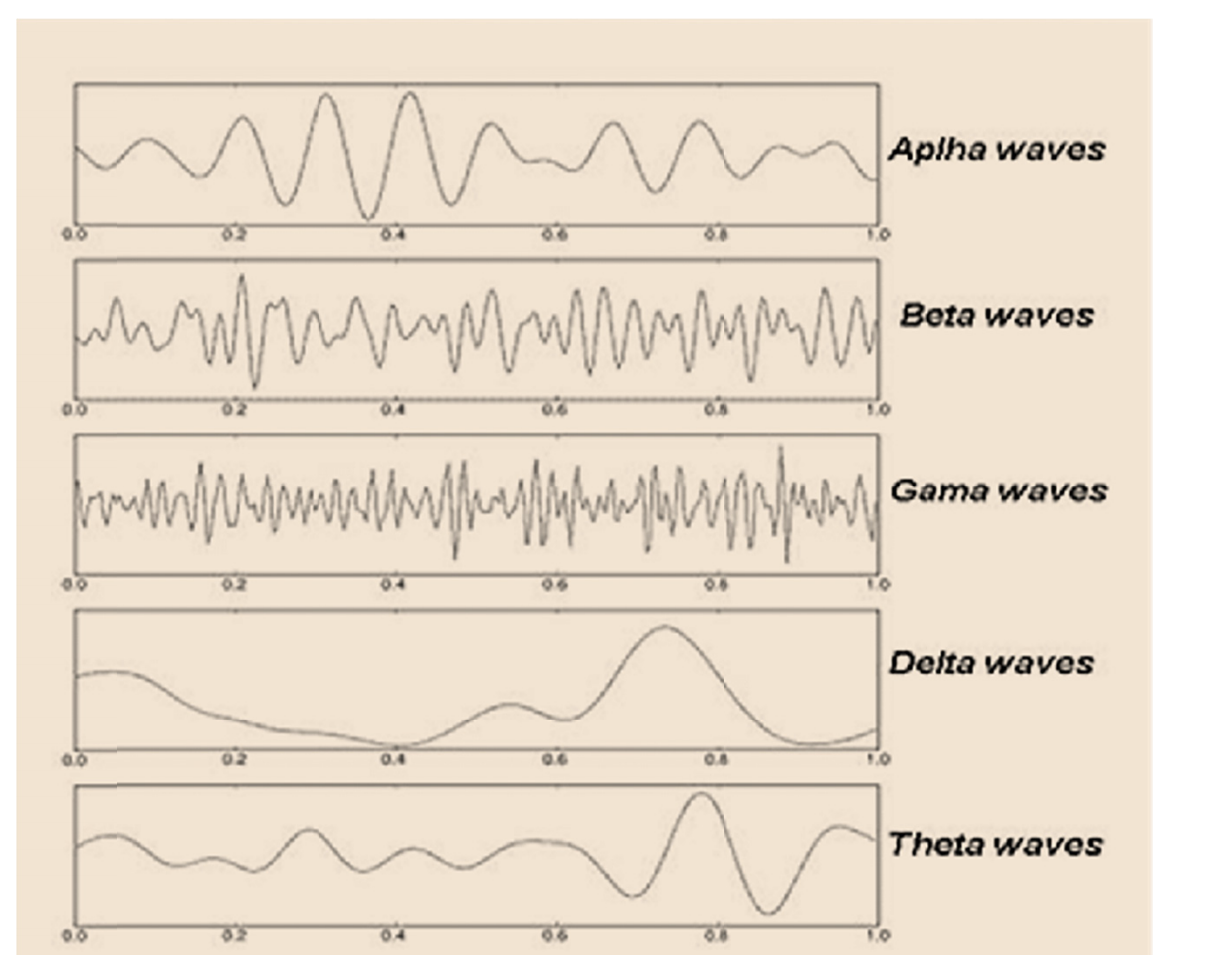
\includegraphics[scale=0.8]{waveforms}\\
		Виды волн головного мозга \cite{41}
	\end{center}
	\section*{Существующие методы выявления и устранения артефактов}
	\addcontentsline{toc}{section}{Существующие методы выявления и устранения артефактов}
	В данной секции будет рассмотрены актуальные методы, часто применяющиеся для выявления и устранения артефактов в данных ЭЭГ. Методы можно разделить на несколько семейств:
	\begin{enumerate}
		\item Основанные на решении задачи Blind Source Separation
		\item Методы, основанные на сконструированных признаках - слепках сигнала
		\item Восстановление сигнала без артефактов с помощью автоэнкодеров
		\item Методы, исследующие графовую структуру ЭЭГ
	\end{enumerate}
	\section*{Известные виды артефактов}
	\addcontentsline{toc}{section}{Известные виды артефактов}
	Существует множество видов артефактов в ЭЭГ, наиболее частые их виды представлены ниже:
		\begin{enumerate}
		\item Связанные с сокращением мышц
		\item Связанные с движением глаз
		\item Связанные с активностью сердца
		\item Связанные с морганием
		\item Связанные с электродами и силовыми линиями
		\item Связанные с выделением пота
		\item Связанные с челюстной активностью
		\item Сторонние шумы (например, звонок телефона)
	\end{enumerate}
	И их иллюстрации на ЭЭГ:\\
	1) Моргание \\
	2) Движение глаз\\
	3) Мышечные артефакты\\
	4) Сердечные артефакты\\
	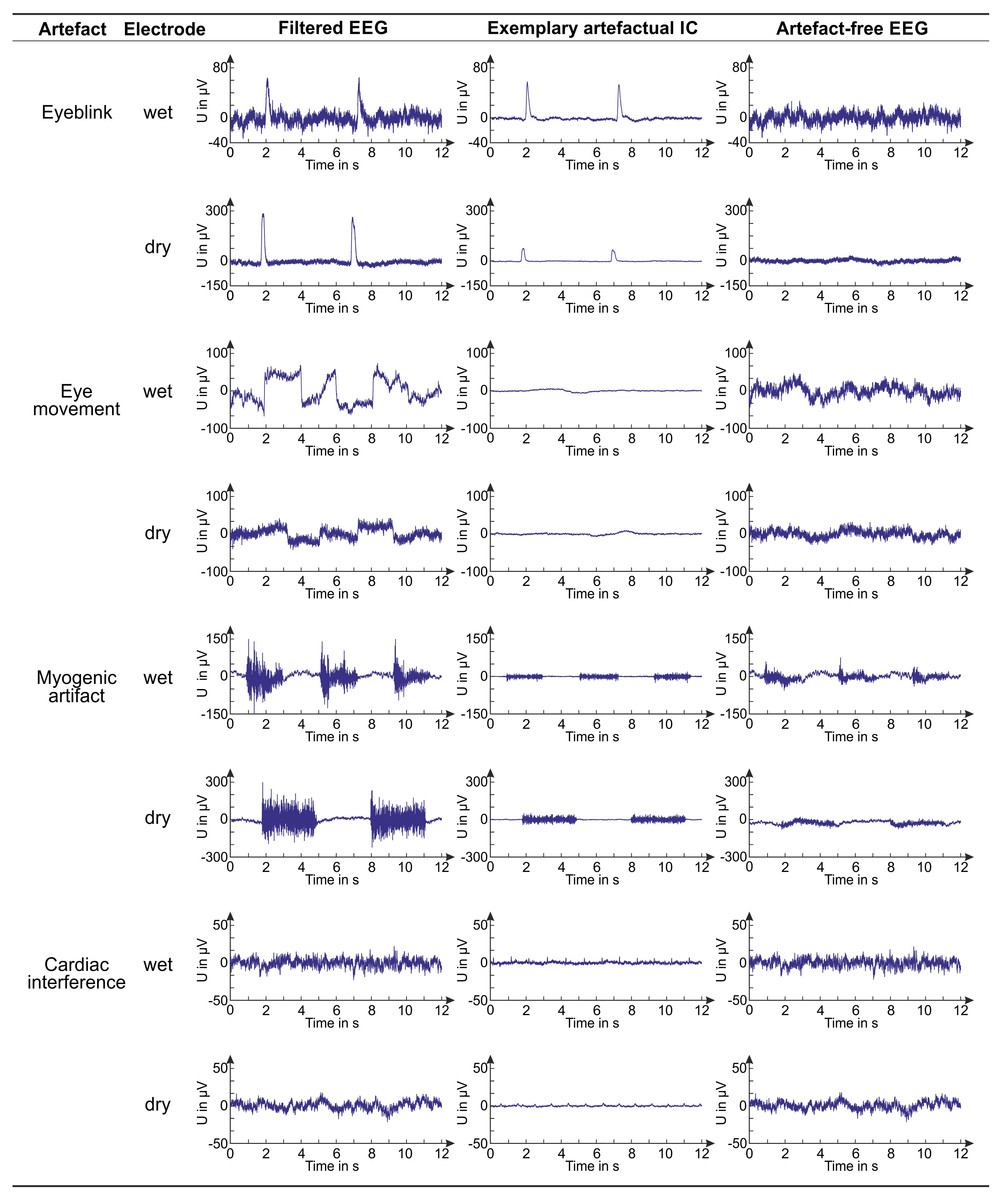
\includegraphics[scale=2]{artifact_types.jpg}\\
	\begin{center}
		Виды артефактов, их соответсвующие независимые компоненты и очищенный сигнал  \cite{30}
	\end{center}
	Примеры артефактов на ЭЭГ, с разбивкой на сигналы с различных электродов:\\
	1) Сокращение мышц и активность сердца.  Мышечный лучше всего заметен в левом височном регионе. Сердечные шумы лучше всего заметны в заднем регионе. \cite{31}:\\
		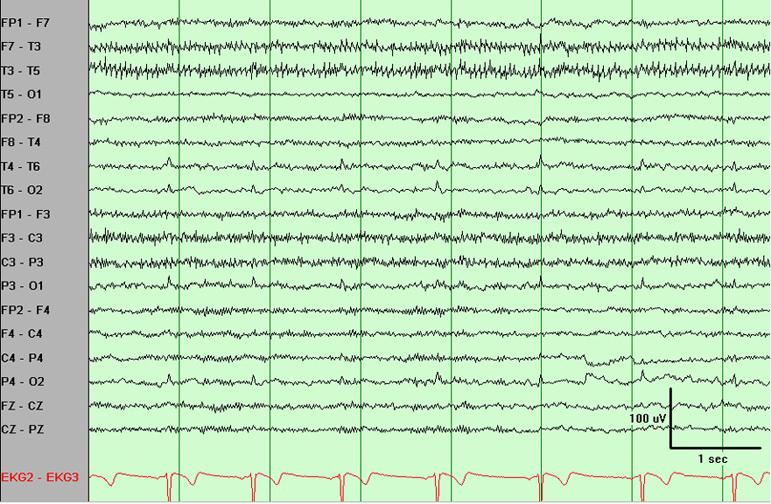
\includegraphics[scale=1]{muscle_artifact.jpg}\\
	2) Движения  глаз. Артефакты такого рода заметнее всего в передних электродах и не дальше среднего региона. Фазовые инверсии на боковых фронтальных электродах F7 и F8 имеют противоположную полярность, что указывает на боковые движения глаз. Поскольку роговица заряжена положительно, а сетчатка отрицательно, сторона положительности указывает направление движения глаза. Таким образом, первое движение здесь идёт вправо. \cite{31}
	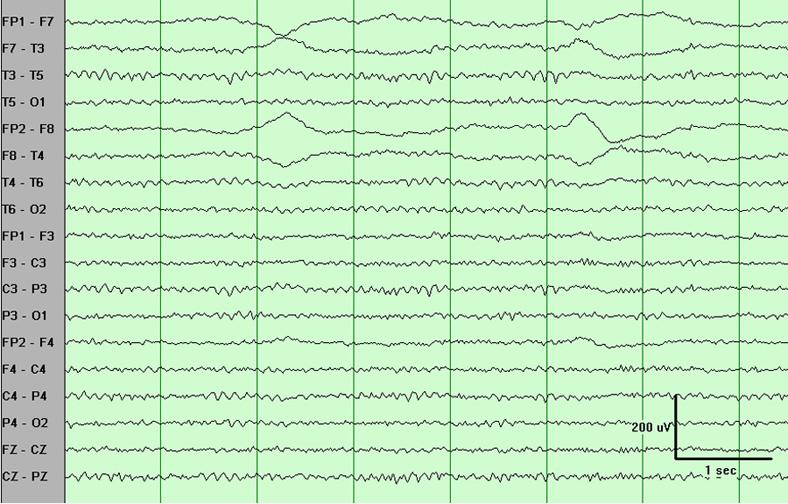
\includegraphics[scale=1]{eye_movement_artifact.jpg}\\
	3) Сердечные сокращения (ЭКГ). Периодические медленные волны лучше всего заметны в средних и задних электродах  T4-T6 и T3-T5. Они явно относятся к ЭКГ. Длительность и морфология импульсного артефакта совпадают, но, как показывает маркер, никакой задержки между ЭКГ и артефактом не происходит. Таким образом, это ЭКГ-артефакт с широкими комплексами QRS. \\
	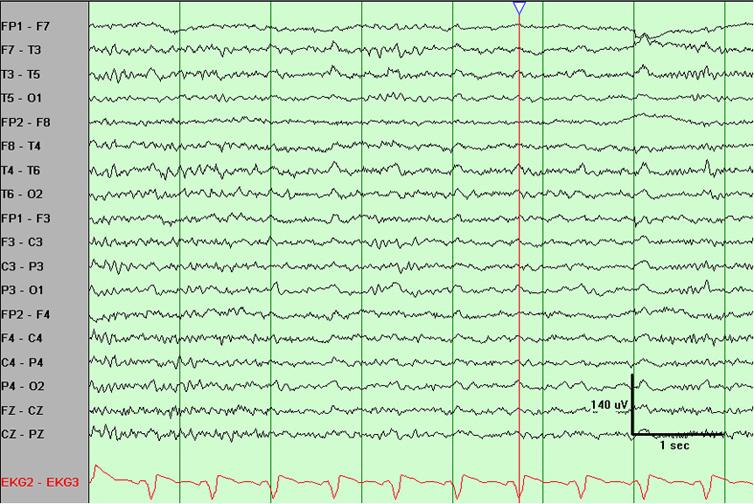
\includegraphics[scale=1]{cardiac_artifact.jpg}\\
	4) Артефакт, вызванный звонком телефона. Он не является типичным в ЭЭГ, поэтому может исказить интерпретацию ЭЭГ.\\
	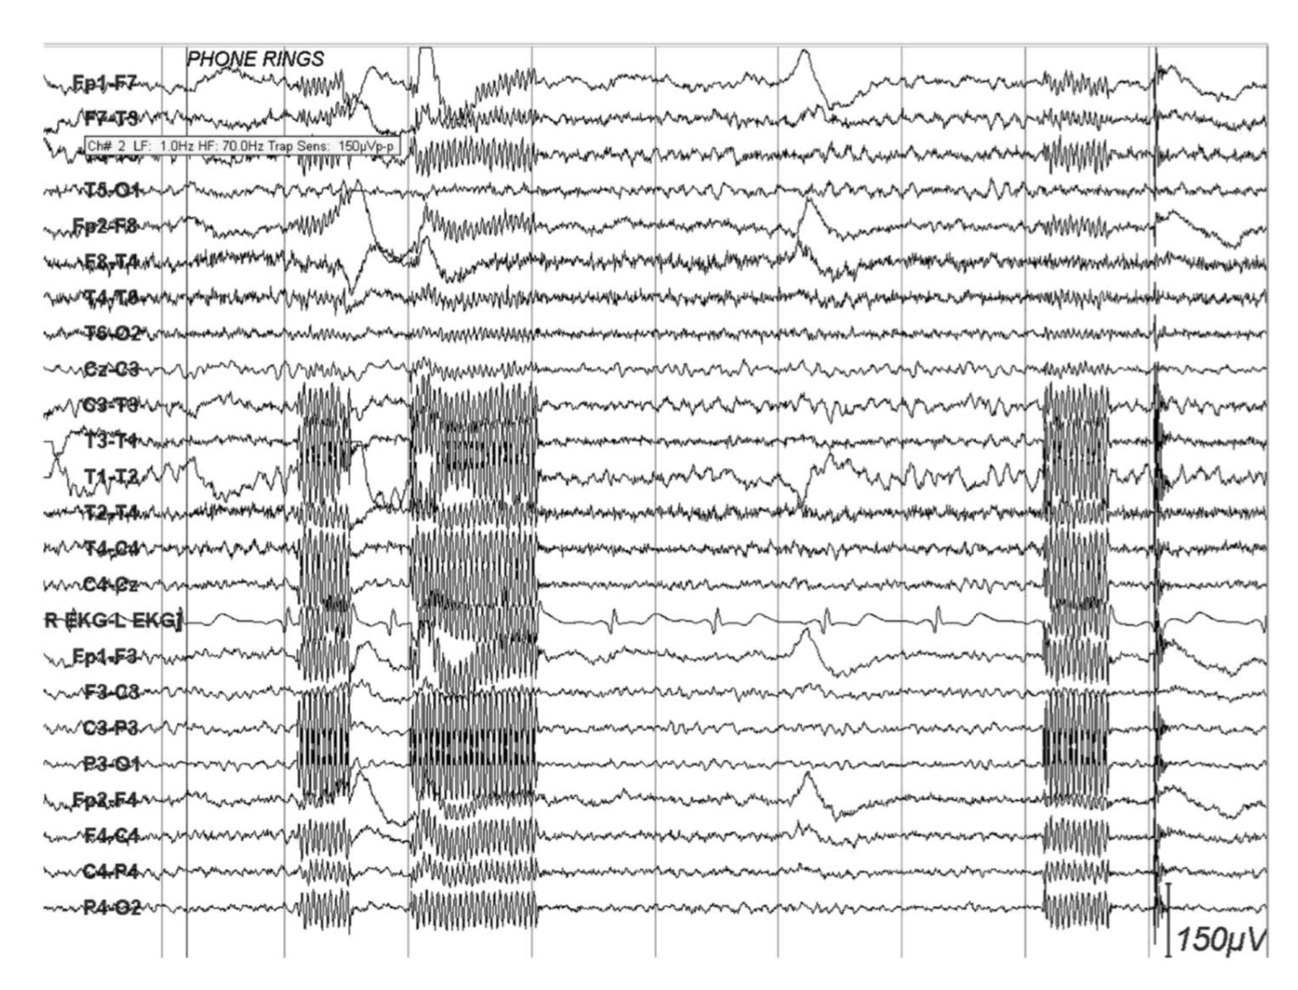
\includegraphics[scale=0.75]{phone_ring}\\
	5) EOG каналы, где левый глаз - это A1, а правый A2 с артефактами вертикального движения глаз. Они могут быть ошибочно интерпретированы, как фронтальная прерывистая ритмическая Дельта активность.\\
	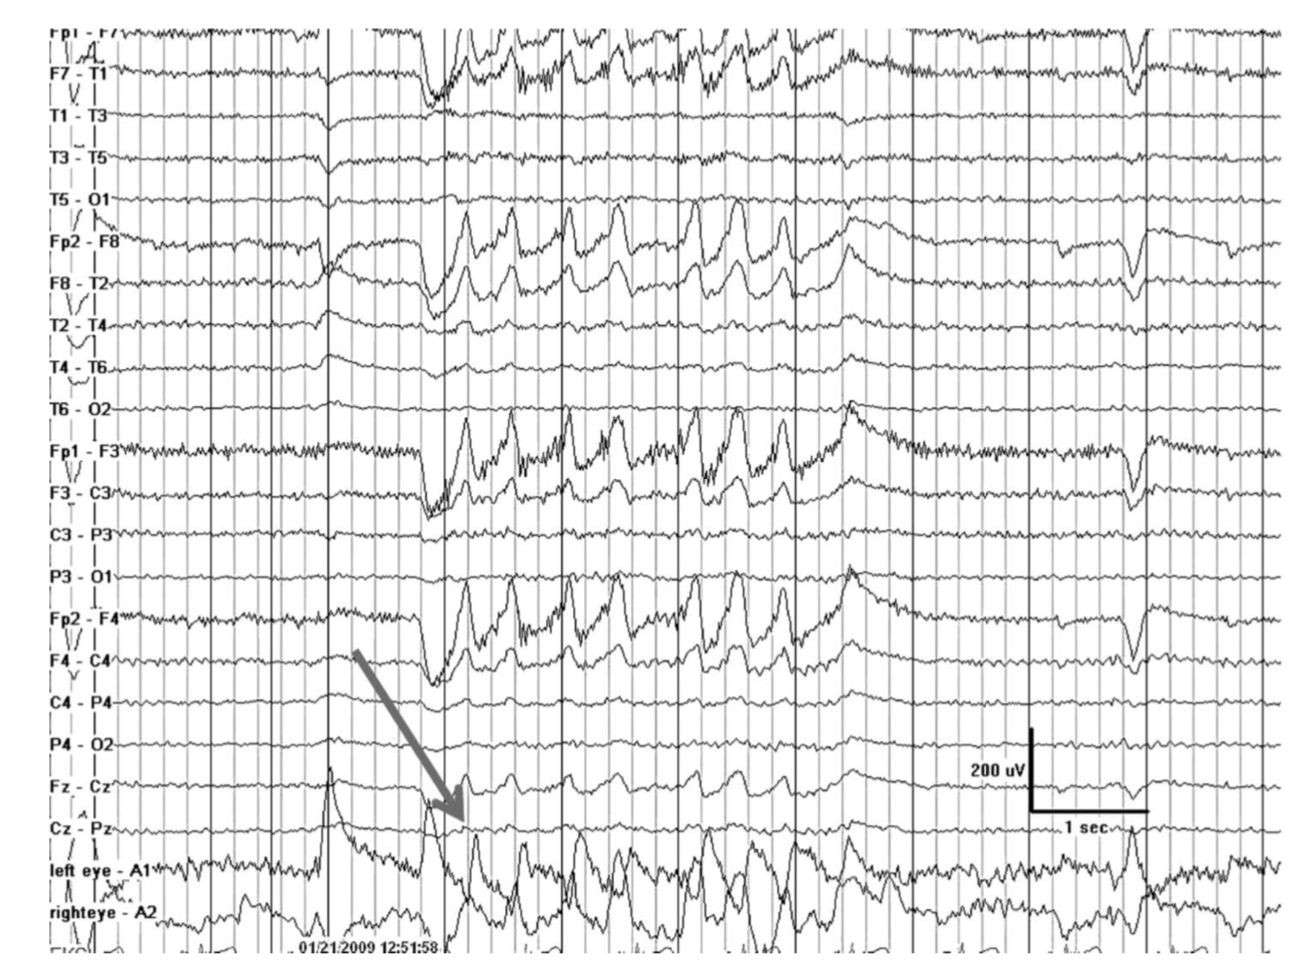
\includegraphics[scale=0.75]{vertical_eye}\\
	6) Артефакт, вызванный выделением пота\\
	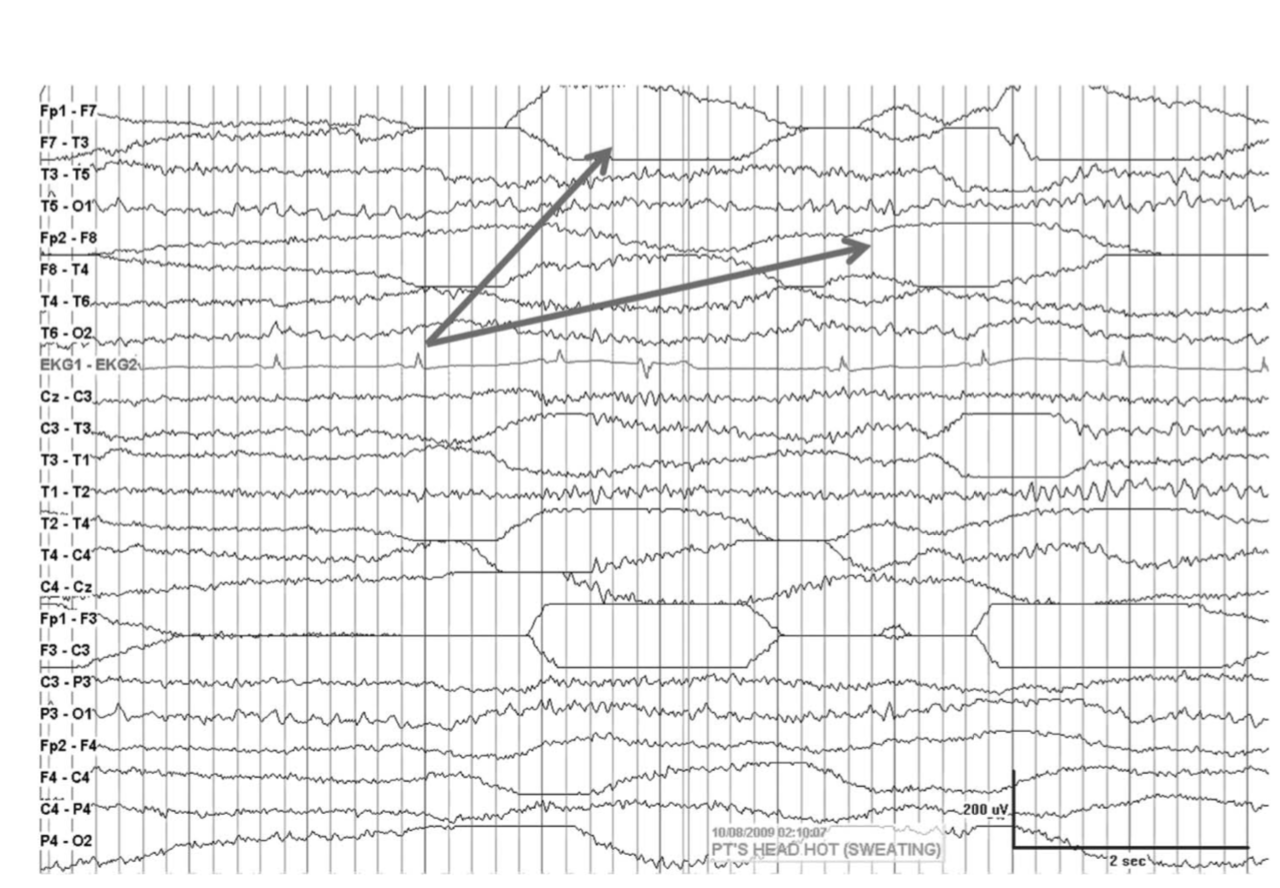
\includegraphics[scale=0.75]{sweat}\\
	7) ЭЭГ с выбросами артефактов, связанных с челюстной активностью: глотание, кашель и жевание.\\
	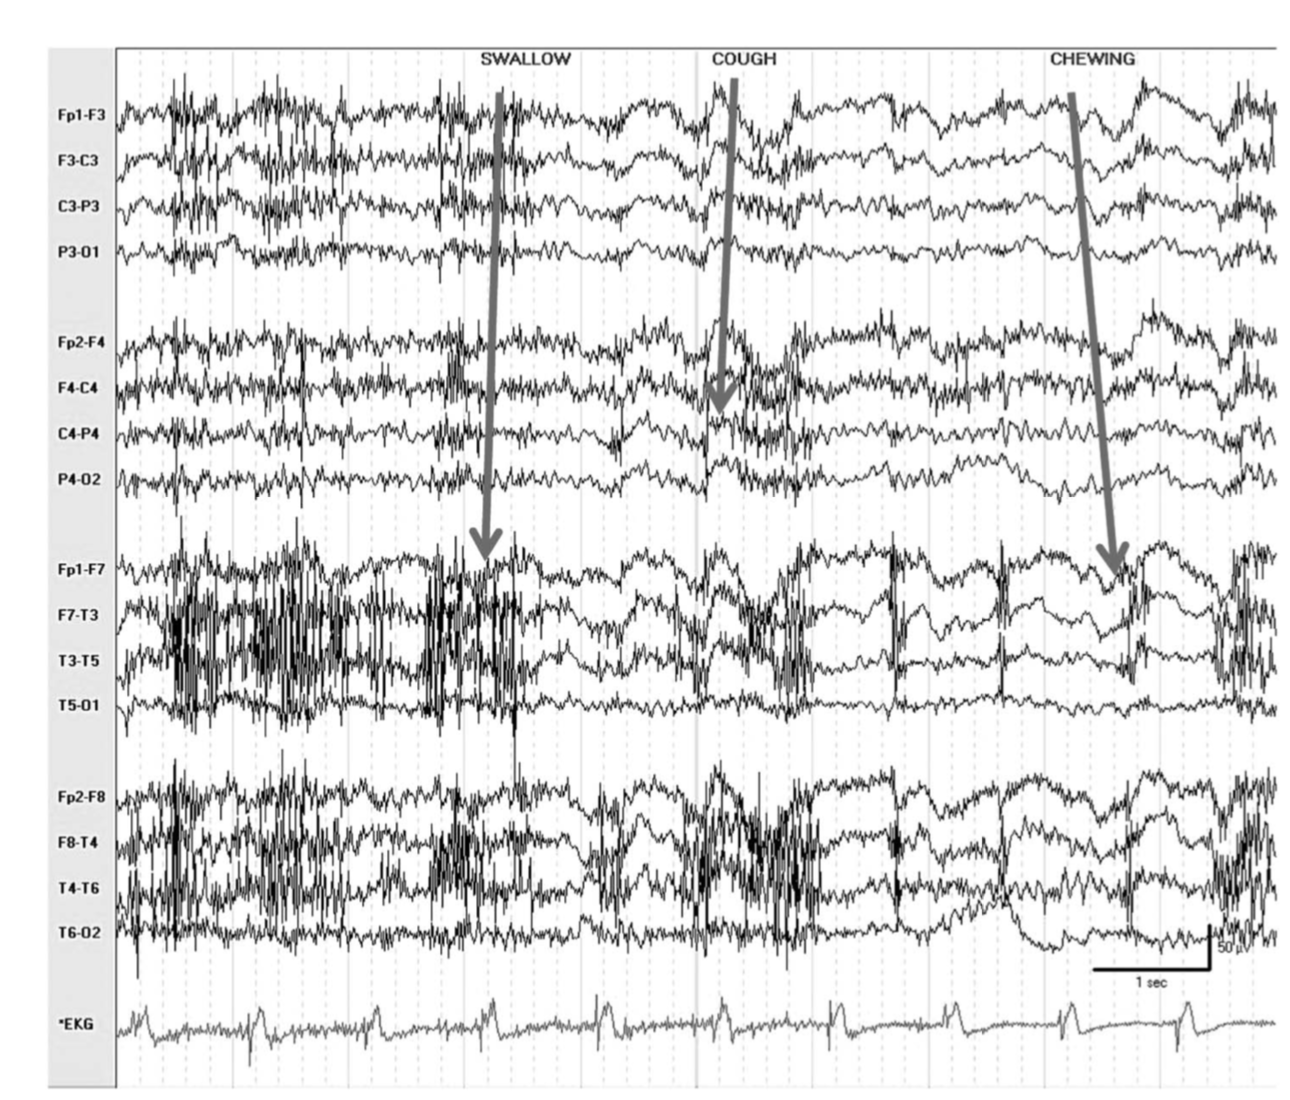
\includegraphics[scale=0.75]{myogenic}\\
	
	\section*{ICA - Анализ независимых компонент и использование слепков для анализа с помощью машинного обучения}
	\addcontentsline{toc}{section}{ICA - Анализ независимых компонент и использование слепков для анализа с помощью машинного обучения}
	\subsection*{Общее описание подхода}
	С помощью этого метода, данные ЭЭГ, в которых содержатся артефакты, разбиваются в набор сигналов с источников, чья статистическая независимость максимизируется, основываясь на некоторых предположениях, одно из которых состоит в том, что большинство нецеребральных вкладов в смешанные сигналы независимы от нейронной активности \cite{43}. Тем не менее, изъятие стереотипных и не стереотипных артефактов обычно требует время-затратного визуального исследования разделённых независимых компонент (IC - individual channels, дальше будем их так обозначать для краткости) человеком, обладающим требуемыми компетенциями. Только после человеческого вмешательства, на которое могут влиять субъективные факторы, есть возможность получить IC, которые относятся непосредственно к активности мозга для дальнейшего анализа.
	
	В работе \cite{30} предлагается использовать SVM для автоматической классификации каналов, чтобы выделить те, в которых нет артефактов четырех видов: моргания, движения глаз, мышечной активности и сердечных артефактов, чтобы восстановить по ним исходный сигнал ЭЭГ. Для этого используются вручную составленные признаки, как указано выше, то есть работа является комбинацией походов 1 и 2. Для каждого вида артефактов обучается своя SVM. Метод основан на следующих предположениях:
	\begin{enumerate}
		\item Вклады, не связанных с активностью мозга сигналов в ЭЭГ независимы от нейронной активности, следовательно, они могут быть отделены, используя подход слепого разделения такой как ICA.
		\item Для большого количества физиологических артефактов, IC, основанные на них характеризуются стереотипными признаками в гиперпространстве параметров
		\item В то время, как одного признака может быть недостаточно чтобы отделить артефактные каналы от других, комбинация нескольких признаков может эффективно достичь этого
		\item Нелинейные методы классификации могут быть более мощными, чем линейные при решении задачи выделения артефактов
	\end{enumerate}
	\subsection*{Данные ЭЭГ}
	В работе использовались данные, полученные с помощью коммерчески доступного униполярного усилителя сигнала (RefaExt; Advanced Neuro Technologies B.V., Enschede, Netherlands) с частотой 1024 записи в секунду. Чтобы оценить разницу в качестве метода при использовании разных типов электродов (влажных и сухих) и их количества, использовались данные, полученные с помощью обычных мокрых шапочек и сухих - нового вида.
	Также были записаны ЭЭГ для каждого вида артефактов, за исключением сердечных, т.к. нет возможности спровоцировать их намеренно, поэтому в их случае использовались данные из других артефактов.
	\subsection*{Предобработка данных и описание метода}
	Сначала, все записи были прошли через полосовой фильтр с обрезанием частот на 0.3 и 100 ГЦ. Применён заграждающий фильтр на 50 Гц чтобы устранить вмешательство силовых линий. Также, применены Хэмминговские оконные sinc-фильтры FIR с помощью firfilt плагина EEGLAB. Плохие каналы, например, те, в которых есть изоэлектрическое насыщение или имеющие излишние артефакты, или же зашумленные более 50\% времени, были определены с помощью экспертов и исключены из анализа.
	
	Далее, очищенные данные были обработаны с помощью анализа главных компонент (PCA) и разложены через ICA. После, были расчитаны слепки IC, используя набор некоторых признаков. Далее, отдельные бинарные классификаторы SVM с нелинейными радиальными функциями были обучены для каждого вида артефактов. Был разработан подход, который определяет и отвергает четыре физиологических артефакта независимо и совместно. Классификаторы тестировались на раздельных IC-слепках полностью автоматически, прошли кросс-валидацию на разных комбинациях случайно выбранных обучающих и тестовых выборках. Статистическая валидация проходила с помощью экспертной разметки.
	
	Оценка качества восстановленных сигналов без артефактов проходила с помощью визуальной оценки и сравнения отношения сигнала к шуму (signal-to-noise ratio - SNR) до и после удаления артефактов.
	\subsection*{Разложение данных с помощью ICA}
	Благодаря объёмной проводимости, сигналы ЭЭГ замеренные на коже головы, получаются из множества мозговых и немозговых источников электрической активности. Исходя из того, что электрические сигналы суммируются в каждой точке размещения электродов без задержки по времени, этот процесс может быть смоделирован линейной одновременной смесью. ICA - это техника слепого разделения источников, которая широко применяется в обработке смеси многомерных сигналов. ICA оценивает статистическую независимость источников сигналов линейно смешанных в нескольких пространственно распределенных записях и реконструирует их временные ряды. Считается, что каждый артефакт независим от сигналов мозга и других артефактов, влияющих на смеси данных. Таким образом ICA - это рабочий метод, чтобы извлекать временные ряды артефактов из ЭЭГ.
	
	Условием правильного применения ICA является то, что смесь данных, смоделированная в виде матрицы, должна считаться неизменной во время записи. Это условие связано с предположением, что смешанные сигналы являются стационарными. Однако физиологические и артефактные сигналы часто производят смеси многомерных сигналов, которые являются нестационарными, поэтому их пропорции в смеси могут изменяться с течением времени. Тем не менее, предположение о стационарности сигнала удовлетворяется при анализе коротких сегментов сигнала (например, записей малой длительности).
	С другой стороны, анализ коротких сегментов сигнала может предотвратить разделение большого числа IC. Чтобы преодолеть эту проблему, был проведен анализ главных компонент (PCA) для уменьшения размерности данных перед применением ICA. Таким образом, возможно было бы выполнить ВСА на сегментах ЭЭГ достаточно коротких, чтобы считаться стационарными, а также получить достаточно большое количество IC. Учитывая кратковременность записи ЭЭГ, был применен ICA ко всему предварительно обработанному временному ряду ЭЭГ и предполагается, что условие стационарности сигнала выполнено.
	Другие работы, в которых используется ICA: \cite{32} - набор данных ICA, который размечается с помощью краудсорсинга, а в качестве основных признаков идут PSD, визуализация временного ряда и визуализация в виде тепловой карты активности сенсоров для каждой из независимых компонент. Он достаточно крупный, но его явный минус состоит в том, чтобы применить модель, обученную на его признаках, необходимо восстановить эти же признаки и в том же формате, как они описаны в датасете, что зачастую является довольно затруднительным, т.к. там применяются показатели, специально подобранные под данные, вроде тепловой карты размером 32x32.\\
	Аналогичный с \cite{30} подход применяется в более ранней работе \cite{33}, где так же строится ICA и применяются слепки сигналов в качестве признаков для классификатора - там же применяются и SVM.
	\section*{Слепки сигналов - вручную составленные признаки, содержащие информацию о сигнале}
	\addcontentsline{toc}{section}{Слепки сигналов - вручную составленные признаки, содержащие информацию о сигнале}
	Исходя из представления о том, что каждый сигнал (а следовательно, и каждый артефакт) характеризуется уникальным ансамблем временных, пространственных, спектральных и статистических признаков, для каждого канала вычисляются признаки, которые охватывают свойства сигнала в четырех областях. Ожидается, что каналы, содержащие один и тот же тип артефакта, будут иметь сходные значения и, следовательно, будут иметь сходный слепок. Некоторые признаки относятся к ранее введенным мерам специфических артефактов, таким как моргания и движения глаз, в то время как другие признаки являются новыми и специально разработаны для обнаружения мышечного и сердечного шумов. Статистические характеристики используются для идентификации конкретных форм сигналов или структуры в отдельных каналах.
	Временные и пространственные характеристики основаны на нормализованных весах каналов для увеличения различного вклада отдельных каналов в записанные наборы данных ЭЭГ. Все объекты представлены на Полярном графике, где каждая ось соответствует отдельному объекту, значение которого варьируется от 0 до 1. Некоторые характеристики варьируются от 0 до 1 по определению (например, CIF и MIF), в то время как другие нормируются между 0 и 1 с помощью различных методов.\\
	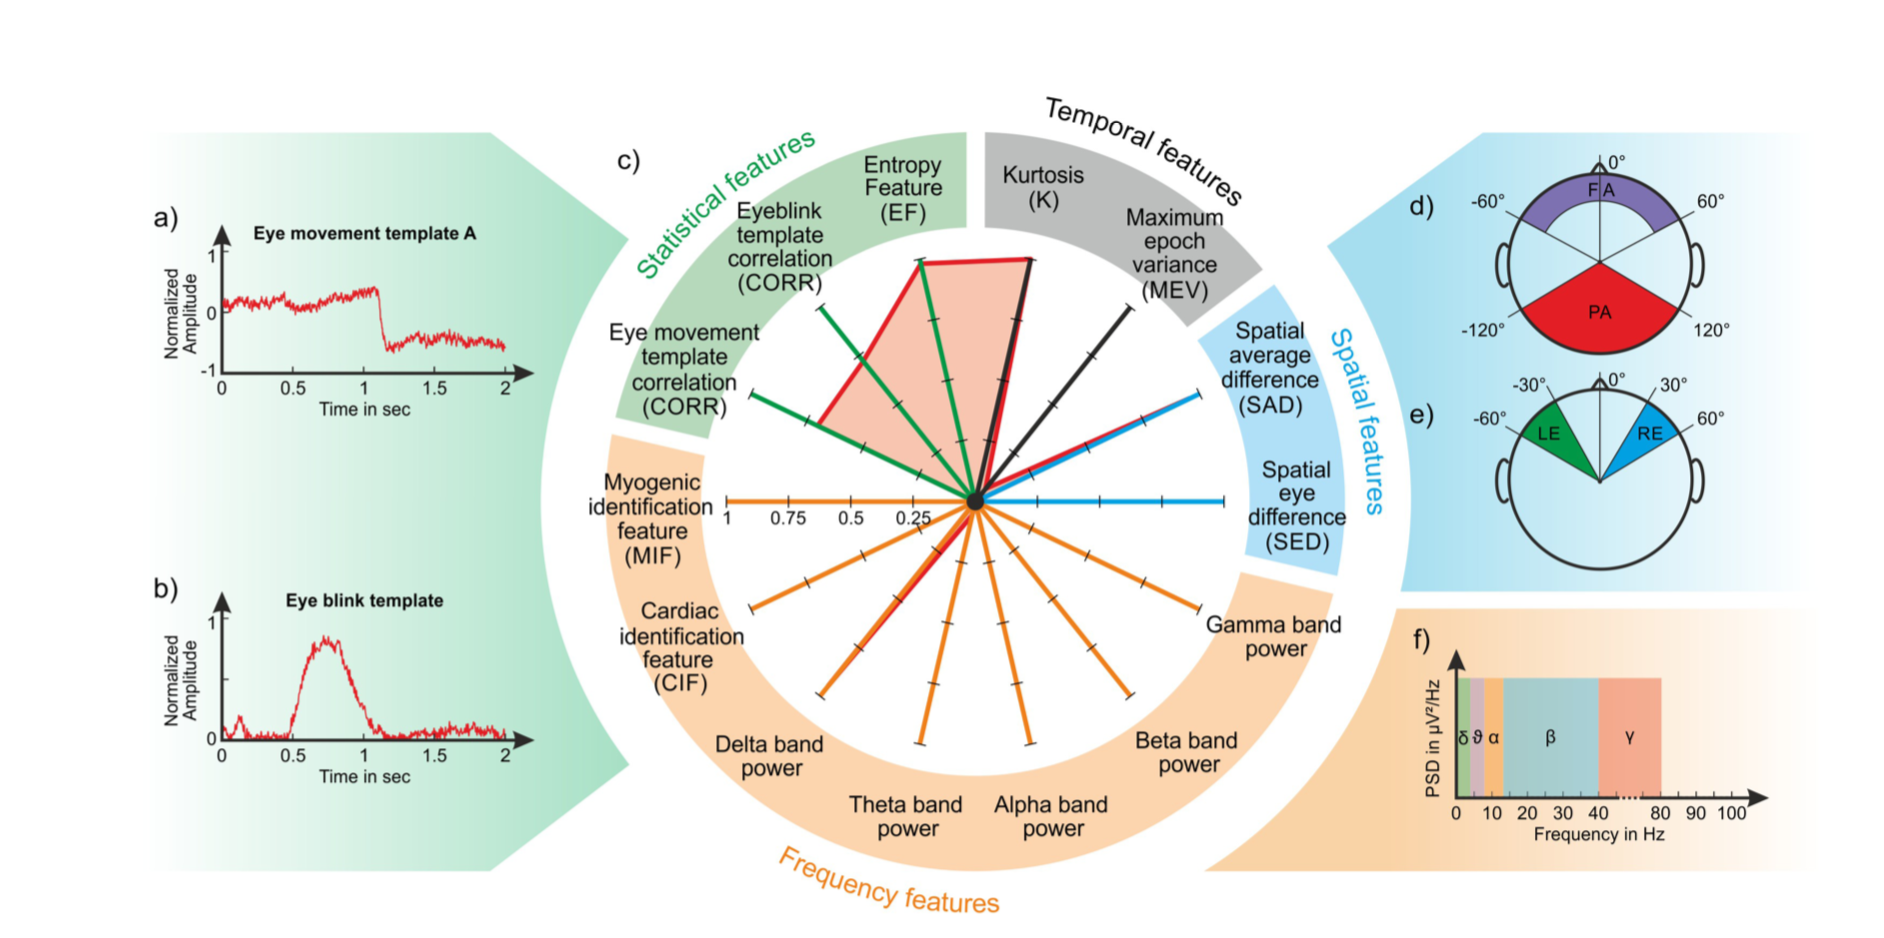
\includegraphics[scale=0.5]{features.png}\\
	\subsection*{Временные признаки}
	Последовательные эпохи по 5 секунд с перекрытием в одну секунду используются для сегментации временного хода отдельных ИС для вычисления двух временных характеристик.
	
	Временной эксцесс (Temporal Kurtosis):
	$$
	K = \frac{1}{m}\sum_{e=1}^{m}(\frac{\frac{1}{n}\sum_{i=1}^{n}(s_{e,i} - \bar{s_e})^4}{(\frac{1}{n}\sum_{i=1}^{n}(s_{e,i} - \bar{s_e})^2)^2} - 3) 
	$$
	где параметры $s_i$ обозначают $i$-е из n выборок данных в векторе данных эпохи e, а m-число эпох в ходе времени канала. Чтобы минимизировать влияние дрейфов и смещений сигналов, для каждой эпохи перед вычислением K вычитается соответствующее среднее значение эпохи. Учитывая, что эксцесс положителен для быстрых изменений амплитуды сигнала, сохраняются только положительные значения K. K особенно подходит для идентификации артефактов, таких как мигание глаз и быстрые движения глаз, которые обычно генерируют краткосрочные изменения амплитуды в сигналах ЭЭГ.
	
	Максимальная дисперсия эпох (MEV). $max()_e$ обозначает максимум во всех значениях эпох.
	$$
	MEV = \frac{max(\frac{1}{n}\sum_{i=1}^{n}(s_{e,i})^2 - (\frac{1}{n}\sum_{i=1}^{n}s_{e,i})^2)_e}
	{\frac{1}{m}\sum_{e=1}^{m}(\frac{1}{n}\sum_{i=1}^{n}(s_{e,i})^2 - (\frac{1}{n}\sum_{i=1}^{n}s_{e,i})^2)}
	$$
	
	Все значения MEV всех каналов нормируются относительно максимального значения. MEV более подходит для обнаружения движений глаз, которые часто имеют более низкую амплитуду и менее краткосрочные изменения.
	
	\subsection*{Пространственные признаки}
	Моргание и движения глаз также характеризуются большими различиями в ЭЭГ, регистрируемой в лобной и височной областях, по сравнению с задними областями. Следовательно, веса каналов, связанных с морганием и движением глаз, показывают характерное распределение на коже головы, которое отражает различные вклады этих артефактных компонент в сигналы ЭЭГ, регистрируемые в различных положениях электродов.
	
	Средняя пространственная разница (SAD) и пространственная глазная разница (SED) расчитываются чтобы оценить пространственное распределение весов каналов на коже головы, группируя веса с учётом $k$ позиций электронов.
	
	Для расчета этих характеристик определены четыре области: 
	\begin{enumerate}
		\item фронтальная область (FA), включающая электроды, угловое положение которых от $0^{\circ}$ до $60^{\circ}$ от медиальной линии и радиальный диапазон которых $\ge 0,4$
		\item задняя область (PA), включающая электроды, угловое положение которых колеблется от $0^{\circ}$ до $120^{\circ}$ от медиальной линии и имеет радиальный диапазон 1
		\item левая область (LE), включающая электроды, угловые положения которых варьируются от $-60^{\circ}$ до $-30^{\circ}$.
		\item правая область (RE), включающая электроды, угловые положения которых варьируются от $30^{\circ}$ до $60^{\circ}$.
	\end{enumerate}
	Пространственная средняя разница (SAD) предназначена для обнаружения мигания глаз и вычисляется в соответствии со следующим равенством:
	$$
	SAD = |\frac{1}{k}\sum_{e=1}^{k}a_{k, FA}| - |\frac{1}{k}\sum_{e=1}^{k}a_{k, PA}|
	$$
	где $a$-вектор весов каналов в положениях $k$ электродов в FA и PA.
	
	Перед расчетом SAD, мы оцениваем, что колебания веса за головы действительно из-за морганий глаз. Во-первых, мы проверяем разницу между дисперсией, связанной с весами передних электродов и дисперсией, связанной с весами задних электродов. Если эта разница $\le0$, это означает, что SAD из-за заднего источника, а не от моргания. В этих случаях, SAD равен 0. Во-вторых, мы сравниваем знаки средних весов в LE и RE. Если они имеют разные знаки, это означает, что есть чистое горизонтальное движение глаз (другой артефакт) и SAD становится равным 0. Во всех остальных случаях SAD рассчитывается по формуле выше.
	
	Пространственная глазная разница (SED) оценивает разницу между весами каналов в областях LE и RE для обнаружения горизонтальных движений глаз.
	$$
	SED = |\frac{1}{k}\sum_{e=1}^{k}a_{k, LE}| - |\frac{1}{k}\sum_{e=1}^{k}a_{k, RE}|
	$$
	
	где, опять же, $a$ - вектор весов каналов в положениях $k$ электродов в областях LE и RE. Чтобы убедиться, что изменения веса действительно вызваны движениями глаз, мы сравним знак средних весов в областях LE и RE. Если средние веса имеют один и тот же знак, SED не обусловлен движениями глаз, и равен 0. Во всех остальных случаях, SED рассчитывается по формуле выше. Наконец, SAD и  SED нормированы относительно максимальных значений SAD и SED всех каналов.
	
	\subsection*{Спектральные признаки}
	PSD в пяти основных диапазонах ЭЭГ: учитывая, что спектральная плотность мощности (PSD) обеспечивает компактное представление распределения энергии сигнала ЭЭГ, для каждого канала вычисляется среднее значение PSD в следующих частотных диапазонах: Дельта-диапазон [0,3-4] Гц, тета-диапазон (4-8) Гц, Альфа-диапазон (8-12) Гц, бета-диапазон (12-40) Гц, гамма-диапазон (40-100) Гц. Пять частотных характеристик рассчитываются как среднее значение PSD в определенных частотных диапазонах, нормированное по максимальному PSD во всех диапазонах.
	Функция идентификации сердца - CIF: этот признак предназначен для идентификации каналов, связанных с сердечными помехами, без использования совместно зарегистрированных электрокардиограмм. Гипотеза состоит в том, что канал, связанный с каридопомехами, должен показывать пик, соответствующий частоте сердца субъекта в распределении PSD в полосе частот, определенной в соответствии с условиями записи.  Интересующая полоса частот определяется, как 0,8-1,7 Гц, поскольку она соответствует диапазону сердечных частот от 48 ударов в минуту до 102 ударов в минуту. Этот интервал включает в себя широкий диапазон сердечных частот для взрослого населения в условиях покоя. PSD расчитывается в полосе частот (0,3-8 Гц), которая больше, чем полоса частот, представляющая интерес, и ищется максимальный пик мощности в этом диапазоне. Если максимальный пик мощности не идентифицирован в диапазоне 0,8-1,7 Гц, то анализируемый канал считается не связанным с сердечными помехами, а CIF устанавливается равным 0. Если максимальный пик мощности входит в диапазон 0,8-1,7 Гц, то канал может быть связан с частотой сердечных сокращений, и его временной ряд анализируется. Во-первых, идентифицируются все пики в ряде канала и выбираются те, которые 
	\begin{enumerate}
		\item больше половины средней амплитуды пика всех найденных пиков
		\item которые происходят на расстоянии, соответствующем интервалу между ударами (в выборках), как и ожидалось на основе максимального пика мощности
	\end{enumerate}
	Функция идентификации сердца (CIF) затем вычисляется как:
	$$
	CIF=\frac{N_{fcp}}{N_{ecb}}
	$$
	Где $N_{fcp}$ число пиков во временном ряде канала, удовлетворяющих условиям 1 и 2, а $N_{ecb}$ – число ожидаемых сердечных сокращений на основе найденного максимального пика мощности в интересующей полосе частот (0,8-1,7 Гц). Если анализируемый канал - это кардиальный артефактный компонент, то CIF должна быть близка к 1. Учитывая, что CIF может варьироваться от 0 до 1, нормировки не требуется.
	
	Миогенная идентификация - MIF: хотя некоторые исследователи наблюдали загрязнение ЭМГ в ЭЭГ на частотах ниже 20 Гц, миогенные помехи, как правило, имеют частотные составляющие выше 20 Гц. Поэтому для каждого канала мы рассчитываем PSD в двух частотных диапазонах: 0-20 Гц ($PSD_{0-20}$) и 21-100 Гц ($PSD_{21-100}$).
	Если $PSD_{0-20}$ больше $PSD_{21-100}$, то мы считаем, что анализируемый канал не содержит миогенных артефактов и MIF имеет значение 0. В противном случае миогенный идентификационный признак (MIF) вычисляется как:
	$$
	MIF=\frac{\sum_{21Hz}^{100Hz}PSD}{\sum_{0Hz}^{20Hz}PSD + \sum_{21Hz}^{100Hz}PSD}
	$$
	Для каналов, содержащих миогенные артефакты, MIF должен быть близок к 1. Учитывая, что MIF может варьироваться от 0 до 1, нормировка не требуется.
	\subsection*{Статистические признаки}
	Рассматриваются два статистических признака: признак, основанный на корреляции между временным рядом канала и шаблоном ожидаемой формы сигнала артефакта, и признак, основанный на оценке структуры временного ряда канала с использованием энтропийной оценки.
	
	Корреляционная характеристика - $CORR$: некоторые артефакты, такие как мигание глаз и движения глаз, демонстрируют характерную форму волны. Были расчитаны характерные шаблоны для миганий и артефактов горизонтального движения глаз, используя один канал из одного набора данных для каждого артефакта (канал и набор данных, где артефакт был наиболее заметен). Шаблоны артефактов были рассчитаны с использованием окон 2 секунды. Для горизонтальных движений глаз использовался только шаблон направления слева направо, потому что шаблон для противоположного направления просто находится в антифазе. Учитывая, что функция  $CORR$ основана на абсолютных значениях корреляции, достаточно использовать один шаблон. Шаблон сравнивается с временным рядом канала, используя движущееся окно 2 С, которое сдвигается на 1 мс до тех пор, пока не будет пройден весь ряд, получая вектор коэффициентов корреляции Пирсона моментов произведения. Затем сохраняются только коэффициенты корреляции с абсолютным значением $\ge 0.65$ и корреляционный признак CORR вычисляется как среднее из сохраненных абсолютных значений корреляции:
	$$
	CORR = \frac{\sum_{i=1}^{N}(r_i)}{N}
	$$
	где $r_i$ - абсолютное значение сохраненного коэффициента корреляции для $i$-го окна канала, а N - общее число сохраненных значений корреляции. Если абсолютное значение корреляции $\ge 0.65$ не найдено, то CORR устанавливается равным 0.
	
	Признак энтропии: энтропия является статистической мерой подобия в данном сигнале и полезна для оценки неравномерности коротких и шумных сигналов биологических систем, включающих как детерминированные, так и стохастические процессы. Артефактные и другие каналы могут быть определены с помощью приближенной меры энтропии $j$-го пятисекундного сегмента $i$-го канала, определяемой следующим образом:
	$$
	H^i = - \sum_{x\in j}p^i_j(x)log(p^i_j(x))
	$$
	где $p^i_j(x)$ вероятность наблюдения значений активности x в распределении активности в $j$-м 5-секундном сегменте  $i$-го канала. После вычисления этих энтропийных мер для всех сегментов и всех каналов мы нормализуем сегментные энтропийные меры на 0-среднее и 1 стандартное отклонение для каждого сегмента во всех каналах. Для каждого канала мы затем вычисляем, сколько энтропийных мер $\ge 1.64$ или $\le -1.64$. Признак энтропии (EF) определяется, как:
	$$
	EF=\frac{N_{sig}}{N_{tot}}
	$$
	где $N_{sig}$ - количество энтропийных мер $\ge 1.64$ или $\le -1.64$, а $N_{tot}$ - общее количество. В случае, если $EF \le 0.2$, EF приравнивается к 0.
	\\
	Подобные признаки используются в работах \cite{36}, \cite{33}, \cite{25}, \cite{16}, \cite{15}
	\subsection*{Оценка качества очистки}
	Эффективность предложенного метода в снижении физиологических помех в записи ЭЭГ оценивалась путем оценки качества реконструированных ЭЭГ-сигналов без артефактов. Для каждого типа артефактов были реконструированы сигналы ЭЭГ для каждого тестового датасета (как влажного, так и сухого) и уровня декомпозиции. Каналы, классифицированные как артефактные с помощью SVM, имевших наилучшую производительность, были проигнорированы, и сигналы ЭЭГ без артефактов в каждой точке расположения электродов были восстановлены путем повторного проецирования всех других каналов обратно в сенсорное пространство. Количество остаточного загрязнения в очищенных ЭЭГ-сигналах оценивали визуальным осмотром и определяли количественно через изменение отношения сигнала к шуму (SNR) между отфильтрованными ЭЭГ-сигналами (т. е. до удаления артефакта) и безартефактными ЭЭГ-сигналами. Для каждого типа артефакта и тестовых датасетов был рассчитан SNR для канала, который показывал наибольшее загрязнение артефактом в отфильтрованной ЭЭГ. Положение выбранного канала должно быть совместимо с типом артефакта. Средние значения SNR не были расчитаны  по всем каналам, потому что каналы, не затронутые артефактом, будет ухудшать эффективность системы шумоподавления. Выбор канала варьировался от одного датасета к другому в зависимости от типа удаляемого артефакта и индивидуальных различий. Уменьшение сердечного загрязнения оценивалось для канала, показывающего наибольшее изменение SNR между фильтрованными и не содержащими артефактов ЭЭГ.
	
	При расчете SNR под сигналом имеется в виду артефакт, а шум - сегмент ЭЭГ, предшествующий артефакту. Это определение подразумевает, что успешное удаление артефакта из ЭЭГ приводит к снижению SNR. Для каждого набора данных SNR был рассчитан по отдельным эпохам, определенным со ссылкам на начало артефакта: сегмент шума $(n)$ включает 200 мс до артефакта, а сегмент сигнала $(s)$ следует за сигналом и имеет длину, которая изменяется между типами артефактов в зависимости от интервала между сигналами. Для каждого сегмента (шум и сигнал отдельно) средняя амплитуда вычитается из каждой временной точки в сегменте.
	$$
	SNR = 10\log_{10}(\frac{\max signal^2 }{\max noise^2})
	$$
	Наконец, SNR каждого канала вычисляется путем усреднения значений SNR, полученных для всех последовательных сегментов шума и сигнала.
	\section*{Глубокий сверточный автоэнкодер}
	\addcontentsline{toc}{section}{Глубокий сверточный автоэнкодер}
	\subsection*{Автокодировщик}
	Автокодировщик (англ. autoencoder) - специальная архитектура искусственных нейронных сетей, позволяющая применять обучение без учителя при использовании метода с обратного распространения ошибки. Простейшая архитектура автокодировщика - сеть прямого распространения, без обратных связей, наиболее схожая с перцептроном и содержащая входной слой, промежуточный слой и выходной слой. В отличие от перцептрона, выходной слой автокодировщика должен содержать столько же нейронов, сколько и входной слой.
	
	Автокодировщик состоит из двух частей: энкодера $g$ и декодера $f$. Энкодер переводит входной сигнал в его представление (код): $h=g(x)$, а декодер восстанавливает сигнал по его коду: $x=f(h)$.
	
	Автокодировщик, изменяя $f$ и $g$, стремится выучить тождественную функцию $x=f(g(x))$, минимизируя какой-то функционал ошибки. $L(x,f(g(x)))$
	
	При этом семейства функций энкодера $g$ и декодера $f$ как-то ограничены, чтобы автоэнкодер был вынужден отбирать наиболее важные свойства сигнала.
	
	Автокодировщик можно использовать для предобучения, например, когда стоит задача классификации, а размеченных пар слишком мало. Или для понижения размерности в данных для последующей визуализации. Либо когда просто надо научиться различать полезные свойства входного сигнала.
	\subsection*{Получение данных}
	Процесс подготовки данных для обучения глубокой нейронной сети включал получение соответствующих исходных данных ЭЭГ, связанных с различными типами шума. В литературе наиболее распространенными источниками шума ЭЭГ являются: моргание глаз; горизонтальное и вертикальное движение глаз, движение рук, механизмы мышц глотания и пищевода, и сокращение нижней челюсти (сжатие челюстей).
	Для сбора электрических сигналов использовался интерфейс мозг-компьютер Brain Wave II EEG 1, разработанный Neurovirtual и состоящий из аппаратного обеспечения с физической системой подключения электродов и программного обеспечения (BW Analysis) для считывания сигналов. Каждый прием шума длился приблизительно 5 минут (включая все вышеупомянутые варианты шума) и имел 25 отдельных каналов, расположенных согласно картинке, за исключением электрода сравнения и трех электродов в области левого глаза, которые не показаны. Настройка оборудования, ориентация добровольцев и дополнительные процедуры добавляли 20-30 минут на сеанс.
	Методология сбора различных типов ЭЭГ шума использовала обучающее видео с визуальными сигналами в форме и цвете для типа действия, которое будет выполняться добровольцами. Например, для моментов, когда они должны моргать глазами, глотать слюну или сжимать челюсти. Эти действия были подробно объяснены каждому добровольцу перед самим экспериментом, а также постоянно напоминались видеоинструкциями во время его демонстрации.\\
	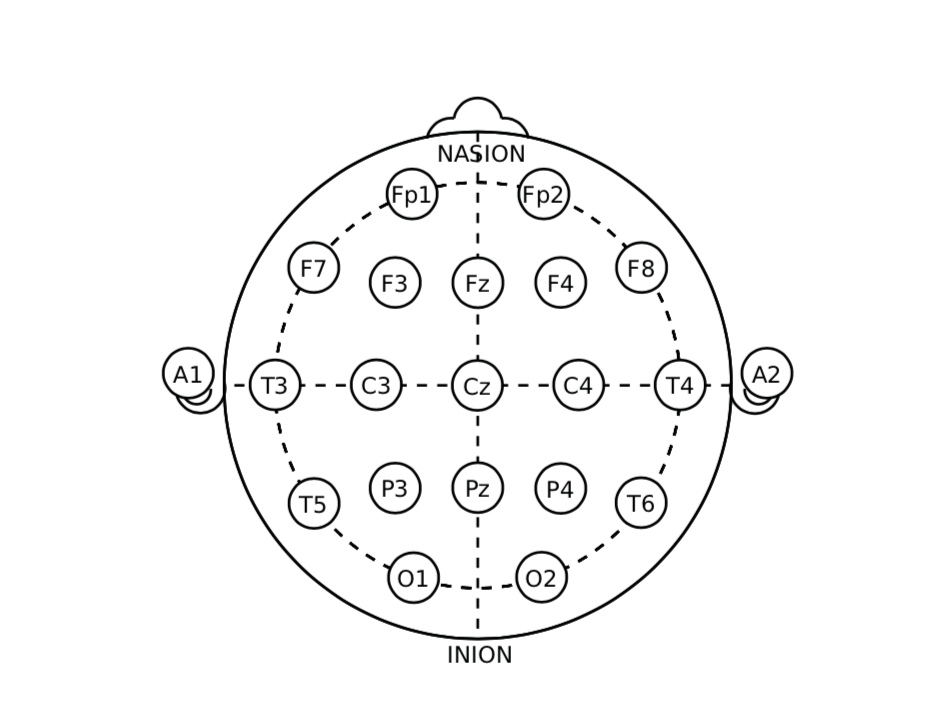
\includegraphics[scale=0.5]{electrodes.png}\\
	\subsection*{Набор данных DEAP}
	Данные описаны в \cite{34}. Для получения чистого сигнала, к которому будут применяться зашумление, используется уже предобработанный набор данных Эти файлы содержат пониженную дискретизацию (до 128 Гц), предварительно обработанную и сегментированную версию данных в Matlab Python/NumPy в форматe pickle и обратно. Эта версия данных хорошо подходит для тех, кто хочет быстро протестировать классификацию или регрессионный метод без хлопот по обработке всех данных в первую очередь. Каждый zip-файл содержит 32 файла .dat (python) или .файлы mat (matlab), по одному на каждого участника.
	Шаги предобработки, которые были выполнены в датасете:
	\begin{enumerate}
		\item Данные были понижены до 128 Гц.
		\item Артефакты ЭОГ были удалены, как и в работе \cite{34}.
		\item Был применен полосовой частотный фильтр с частотой 4,0-45,0 Гц.
		\item Эти данные были усреднены по общей ссылке.
		\item Каналы ЭЭГ были переупорядочены таким образом, чтобы все они следовали Женевскому порядку, как указано выше.
		\item Эти данные были разделены на 60-секундные испытания и 3-секундный предварительный базовый уровень был удален.
		\item Испытания были переупорядочены из порядка презентации в порядок видео (Experiment\_id).
	\end{enumerate}
	\subsection*{Обработка данных}
	После каждого сеанса сбора данных ЭЭГ создавался файл с базовой ЭЭГ, содержащий все типы шума, упомянутые выше. Затем этот файл данных был должным образом сегментирован, чтобы получить отдельный файл для каждого из пяти вариантов шума. Добавление требуемых шумов к бесшумной ЭЭГ позволяет лучше контролировать его проявления. Бесшумные ЭЭГ-сигналы были получены из набора данных DEAP EEG для анализа эмоций (состоящего из 32 испытуемых), с использованием методов предварительной и постобработки авторов датасета, которые визуально не проявляли ни одного из вышеупомянутых типов шума.
	Используя эти два набора данных (DEAP и данные с шумом), можно было получить две версии каждого сигнала (одна бесшумная, а другая с добавлением шума), которые использовались для обучения нейронной сети. Предполагая, что шумовые участки собранной базовой ЭЭГ были более заметны по амплитуде, чем сама информация ЭЭГ, можно было сделать вывод, что, добавляя части собранной ЭЭГ, в которых происходил шум (например, моменты, в которые происходили моргания глаз), добавлялся сам шум.
	
	Сопоставление датасетов: для добавления шума к сигналам из набора данных DEAP были необходимы процедуры обработки, соответствующие их форматам. Сигналы DEAP первоначально имели 32 канала ЭЭГ на субъекта, с метками в соответствии с их эмоциональной оценкой, в то время как база шумов имеет 25 каналов. Сигналы DEAP игнорировали свои эмоциональные ярлыки, поскольку эта информация была неуместна для фильтрации шума. Наконец, были сохранены только каналы, существующие в обоих наборах данных; каналы из базы данных шума, отсутствующие в наборе данных DEAP и наоборот, были отброшены, что привело к окончательному формату 19 каналов на субъекта. Все каналы за исключением А1 и А2, были включены в окончательный 19-канальный формат.
	
	Синтетическая генерация ЭЭГ для увеличения объема данных: для того чтобы нейронная сеть получала достаточное количество данных, необходимых для обучения требуемой функции фильтрации, было необходимо больше данных, нежели данные 32 субъектов. Процесс был основан на восстановлении сигналов с заданной спектральной плотностью мощности (PSD) и проверен с помощью обратной процедуры для получения того же самого временного входного сигнала.
	Математическое обоснование включает в себя общие понятия и формулы преобразования частоты во времени, такие как: вычисление PSD сигнала (чтобы исследовать его частотное поведение и попытаться эмулировать его в синтетических сигналах); вычисление обратного преобразования Фурье (чтобы получить сигнал временной области из сигнала частотной области); генерация случайного распределения из статистических свойств, таких как среднее и стандартное отклонение (полученные из исходного сигнала временной области). Использовались также такие операции, как интерполяция, генерация случайных чисел в интервале и умножение комплексных чисел.
	Следующие шаги были выполнены для каждого канала данных из набора данных DEAP. Каждый канал рассматривался как массив $eeg\_channel[n]$ из $m$ объектов, в котором $n$ - переменная индексации области дискретного времени.
	\begin{enumerate}
		\item Вычисление среднего и стандартного отклонения массива $eeg\_channel[n]$ из DEAP датасета;
		\item Генерация массива $s\_channel[n]$ из $m$ значений белого шума в соответствии с гауссовым распределением среднего и дисперсии, заданным ранее;
		\item Вычисление спектральной плотности мощности (PSD)  $eeg\_channel[n]$ и  $s\_channel[n]$, последующее их умножение для получения результирующего PSD с формой, более близкой к форме ЭЭГ;
		\item Вычисление массива амплитуд $A[n]$ с использованием (1) и результатов шага 3 для каждого образца $k \in [1, m]$;
		\item Назначение случайной фазы $P[k] \in [0, 2\pi]$ для каждого $k \in [1, m]$, т. е. для каждой из полученных амплитуд $A[k]$
		\item Комбинация соответствующих амплитуд и фаз вычисленных в предыдущих шагах с использованием (2) для получения массива $Z[\omega]$, в котором $\omega$ является переменной индексации дискретно-частотной области;
		\item Применение обратного дискретного преобразования Фурье на $Z[\omega]$ для получения сигнала дискретной области времени $z[n]$;
		\item Исправление любого оставшегося несоответствия размерностей в $z[n]$ с помощью применения линейной интерполяции.
		\end{enumerate}
	\begin{align*}
	A[k] = \sqrt{2 PSD_{eeg\_channel}[k] \cdot PSD_{s\_channel}[k]}\\
	Z[\omega] = A[n]\cdot exp(j P[n])
	\end{align*}
	
	К концу этого процесса сигнал $z[n]$ эквивалентен каналу ЭЭГ с точки зрения общей формы и частотного распределения. Поскольку эти данные имели единственную цель эмуляции формы ЭЭГ, а не предоставление реальных клинически валидных данных, этого было достаточно.
	
	\subsection*{Структура нейронной сети}
	
	Глубинные нейронные сети - это искусственные нейронные сети, характеризующиеся многослойной структурой, позволяющей получить большее количество уровней абстракции объектов, чем обычные (неглубокие) сети. Deep Autoencoders (DAEs) - это архитектуры, которые могут изучать статистическую информацию высокого порядка о входных данных и обычно структурированы симметрично относительно их размерности.
	
	Начальные запуски с более простыми архитектурами обычно включали четыре скрытых слоя (2D свертка, отсев, отсев и 2D свертка). Однако результаты обучения на этих начальных этапах не были благоприятными для удаления шума, и его эффективность часто количественно оценивалась с высокими кумулятивными потерями (около 100 \%) в валидационном наборе данных.
	
	Изучив влияние таких параметров, как количество фильтров, условия регуляризации и выбор слоев для использования, была получена структура, показанную ниже, которая выполняли предсказания шумоподавления и были подтверждены с довольно низкими потерями ($< 2\%$).
	
	Во время предварительной репликации декодированного (безшумного сигнала) слоя из входного слоя (шумного сигнала) ожидается, что сеть сохранит модель, необходимую для удаления шума из входного слоя, если таковой имеется.
	\begin{enumerate}
		\item Слой Conv2D выполняет двумерную свертку между двумя последовательными слоями для каждого канала оцениваемой ЭЭГ.
		\item Слой MaxPooling2D концентрирует нейронные выходы из предыдущего слоя в отдельные нейроны следующего слоя, используя максимальное значение первого и таким образом уменьшая размерность после каждой операции.
		\item Слой UpSampling2D увеличивает размерность, чтобы компенсировать эффекты слоя MaxPooling2D, таким образом давая симметричную структуру сети, как и ожидалось от автоэнкодера.
	\end{enumerate}
	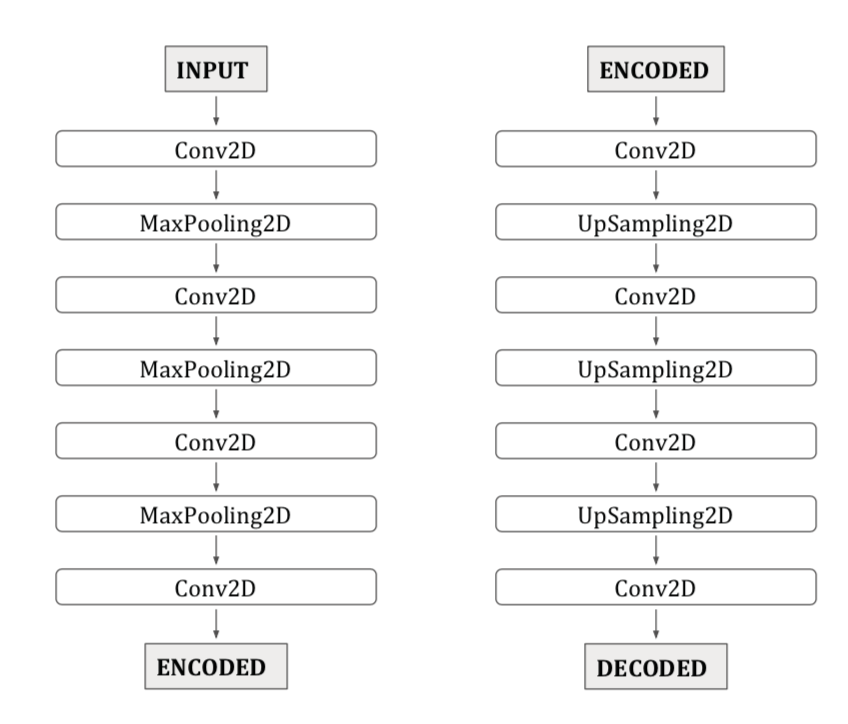
\includegraphics[scale=1]{architecture.png}
	\\
	Поскольку сигналы были на частоте 128 Гц и каждый канал имел длительность 60 секунд, каждый из них содержал 7680 образцов. Каждый объединяющий слой вызывает уменьшение размера, в то время как каждый увеличивающий слой делает противоположное, как было объяснено ранее.\\
	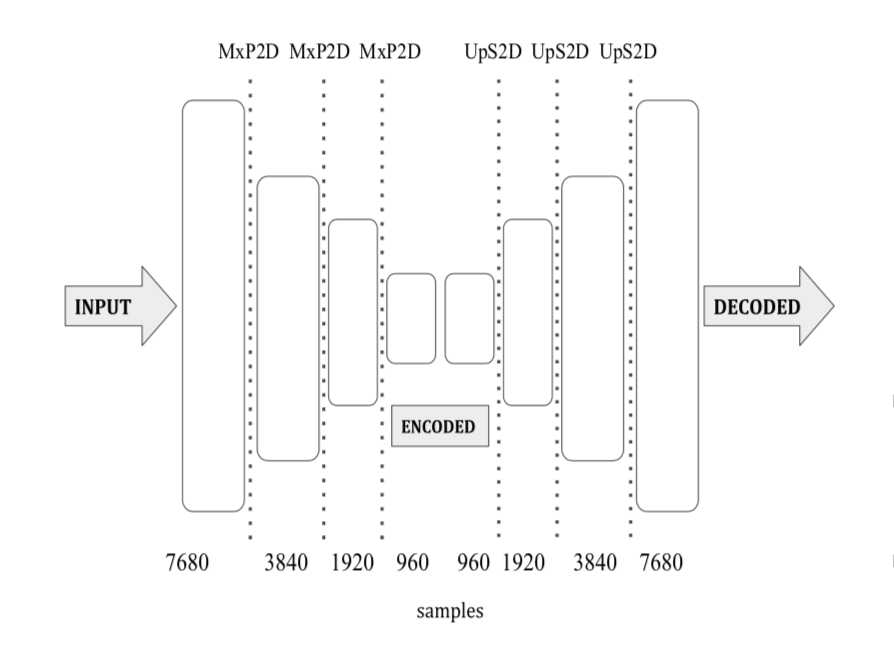
\includegraphics[scale=1]{dimensions.png}
	\\
	\subsection*{Метрика оценивания}
	Метрикой, используемой для оценки, был PSNR (пиковое отношение сигнала к шуму) фильтрованных сигналов, принимая бесшумный сигнал за эталонный. Эта оценка проводилась поканально.
	$$
	PSNR = 10\cdot log_{10} (\frac{MAX^2_I}{MSE})
	$$
	Где $MAX_I$ - максимальное значение амплитуды для бесшумного канала, а $MSE$ - среднеквадратичная ошибка между бесшумным каналом и зашумленным каналом после фильтрации.
	\subsection*{Практическая реализация}
	Сеть была реализована с помощью Keras Deep Learning Library на Python 3.x. Финальная конфигурация:
	\begin{itemize}
		\item Функция активации: $tanh$ - гиперболический тангенс
		\item Размер ядра свертки = 8
		\item Количество фильтров = 100
		\item Без регуляризации в сверточных слоях
		\item Функция потерь: MSE
		\item Оптимизатор: SGD - стохастический градиентный спуск с learning\_rate = 0.01
	\end{itemize}
	Были сформированы группы из 19 каналов (соответствующие одному субъекту) обозначенные, как "записи". Обучение сети с более чем 300 записями 19-канальных сигналов ЭЭГ (уже включавших синтетические данные) представляло собой сложную вычислительную задачу. Из-за ограничений обработки на аппаратном уровне, а также из-за использования большинства альтернатив на программном уровне, вся масса данных не могла быть обработана сразу, т. е. с использованием всех данных для каждой эпохи обучения.
	
	Решение этой проблемы состояло в разделении данных на батчи таким образом, чтобы каждый батч обучал сеть в течение одной эпохи, последовательно, пока все батчи не будут учтены. Один полный цикл был бы учтен, когда все данные прошли бы через сеть, суммируя одну макроэпоху, то есть одну эпоху, которая учитывает обучение заданного количества батчей данных, каждый батч обучал бы одну эпоху за один раз.\\
	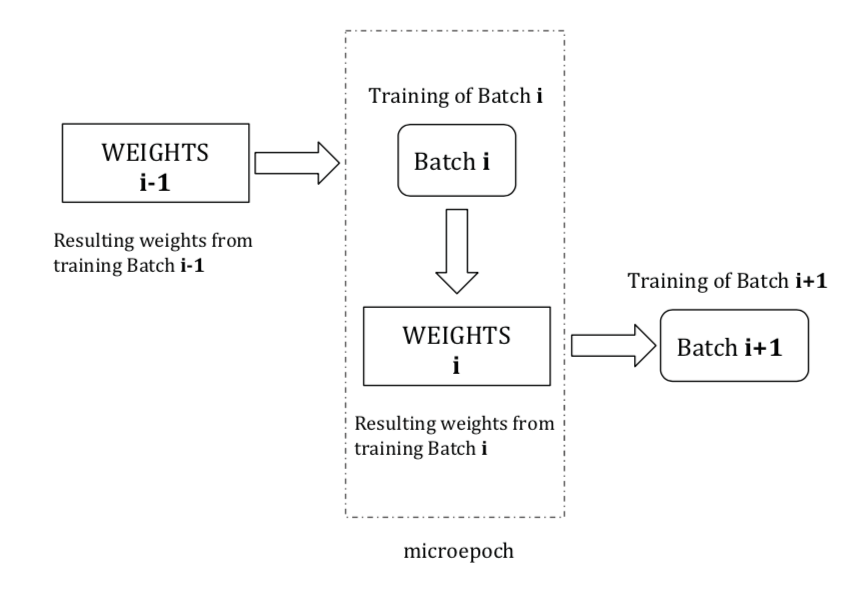
\includegraphics[scale=1]{batch_scheme.png}
	\\
	Таким образом на выходе получался отфильтрованный сигнал.
	\section*{Подходы, основанные на графах}
	\addcontentsline{toc}{section}{Подходы, основанные на графах}
	В работе \cite{29} предложен подход классификации ЭЭГ, основанный на классификации графов. В даннном случае, решается задача бинарной классификаци между двумя классами: нормальная и аномальная ЭЭГ. Полезным является тот факт, что методика, предложенная в данной работе, применима и для выявления артефактов, т.к. сама концепция связности источников сигналов позволяет классифицировать и события.
	\subsection*{Ключевые идеи}
	Ключевые идеи этого исследования заключаются в следующем: \\
	1) взаимодействие
	между областями мозга можно использовать для извлечения полезного
	особенности для классификации аномалий и\\
	2) Особенности из пар области мозга связаны друг с другом.\\
	Используя корреляционную матрицу, можно выразить силу взаимодействия между парами электродов, которая может быть непосредственно отображена на графическое представление: каждый узел является электродом и каждое ребро добавляется, если корреляция достаточно сильна. Это мотивируется пространственным расположением электродов и биологическими механизмами, которые на самом деле включают в себя более одной области мозга одновременно для бытовых задач. Кроме того, по конструкции добавляется ребро к графу тогда и только тогда, когда он является допустимым представлением взаимодействия между парой узлов (т.е. для пары областей мозга), так что для каждого узла механизм "внимания" выполняется на хорошо структурированном и физиологически мотивированном участке\\
	\subsection*{Основные понятия}
	С теоретической точки зрения сети можно моделировать с помощью графов, т. е. абстрактных объектов, представляющих собой совокупность сущностей V (вершин или узлов) и отношений между ними, т. е. ребер, E. В настоящей работе используются атрибутивные графы, G = (V, E), где каждая вершина $v \in V$ помечается вектором значений атрибутов. Кроме того, учитывая вершину  $v \in V$, указывается с помощью
	$N (v) = {u \colon {v, u} \in E}$ окрестность вершины v. Для того чтобы суммировать отношения между вершинами и захватить релевантную информацию в графе, обычно применяется вложение (т. е. преобразование объектов в пространства более низкой размерности)\\
	Пусть имеется граф $G = (V, E)$ с $V$ - множеством вершин и E множеством ребер, тогда
	цель эмбеддинга узлов состоит в том, чтобы обучить функцию
	$f \colon V \to R^k$
	такую, что каждая вершина $i \in V$ сопоставляется K-мерному вектору $\vec{h}$.\\
	Пусть дано множество графов, $\c{G}$, 
	задача эмбеддинга графа состоит в обучении функции $f: \c{G} \to R$ сопоставляет входной граф $G \in \c{G}$ с низкоразмерным эмбеддинговым вектором,$\vec{h}$.
	\subsection*{Механизм внимания и GAT}
	В \cite{29}  применяется эмбеддинги основанные на механизме внимания, как было предложено в \cite{24} путем введения наложенной архитектуры для классификации типа ЭЭГ.
	Определение механизма внимания:\\
	Механизм внимания - это функция $a : R^n \times R^n \to R$ которая вычисляет коэффициенты
	$e_{i, j} = a(\vec{h^l_i}, \vec{h^l_j})$ на парах вершин $i, j$, основанных на признаковом представлении $\vec{h^l_i}, \vec{h^l_j}$ на уровне $l$\\
	Коэффициенты $e_{i, j}$ могут быть рассмотрены, как релевантность признаков вершины $j$ относительно $i$
	\subsection*{Схема эксперимента}
		\begin{itemize}
		\item Многомерные данные разбиты на несколько пересекающихся окон по времени
		\item Каждый ряд из подвыборки используется, чтобы получить кросс-корреляционную матрицу, состоящую из значений корреляции Спирмена между каждым из каналов
		\item Для каждого графа получается GAT-сеть
		\item Эмбеддинг  GAT из  $j$ GAT сети, которая характеризует j-е эмбеддинговое представление соотносится с другим выходом. чтобы получить последовательность GAT эбеддингов на вход для LSTM
		\item Входной набор узловых признаков $\vec{h} = {\vec{h_1},\vec{h_2},\dots,\vec{h_N}}$
		состоит из векторов признаков $\vec{h_i} \in R^F$, где F - количество объектов для каждого узла. В этой статье один вектор признаков составляется из пяти признаков и вычисляется путем извлечения среднего значения мощности для пяти хорошо зарекомендовавших себя частотных диапазонов, такие как Дельта (0,5-4 Гц), тета (4-8 Гц), Альфа (8-12 Гц), бета (12-30 Гц) и гамма (30-100 Гц), в соответствующем окне
	\end{itemize}
	Схему можно увидеть на иллюстрациях:
	\begin{figure}
		\centering
		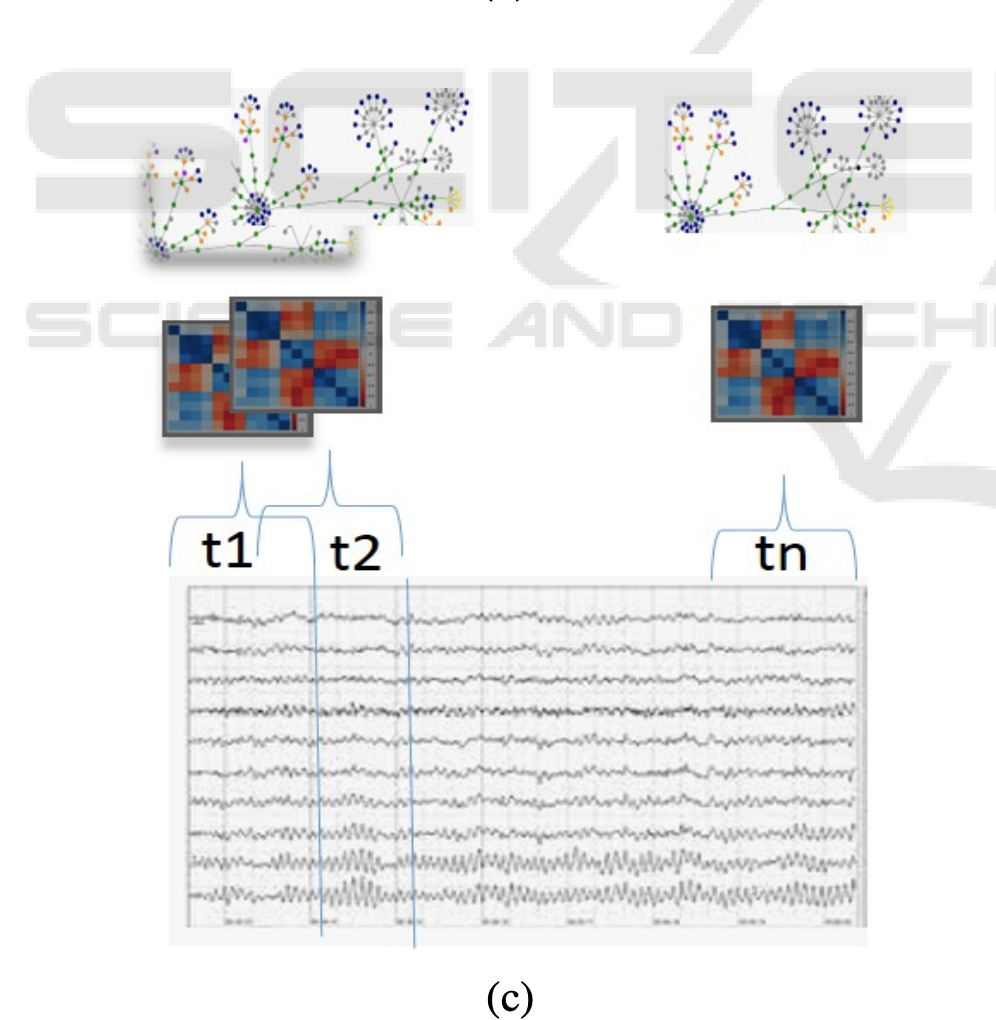
\includegraphics[width=0.7\linewidth]{1_step}
	\end{figure}
	\begin{figure}
		\centering
		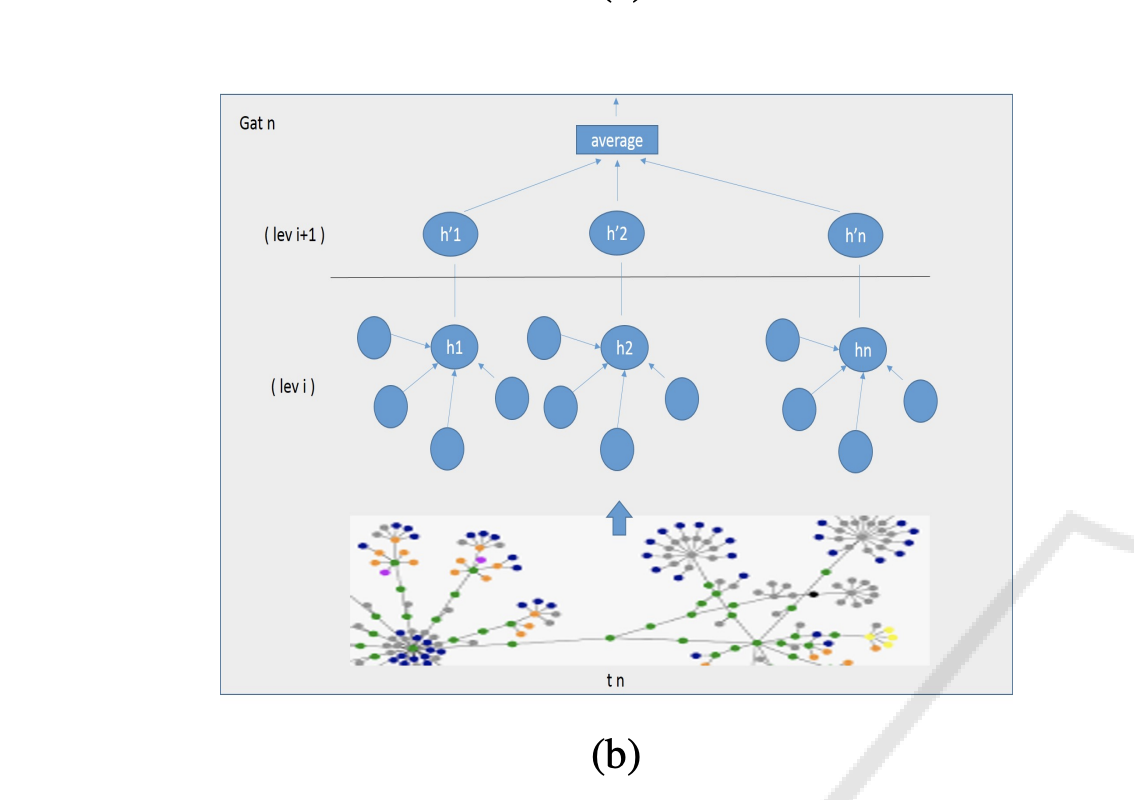
\includegraphics[width=0.7\linewidth]{2_step}
	\end{figure}
	\begin{figure}
		\centering
		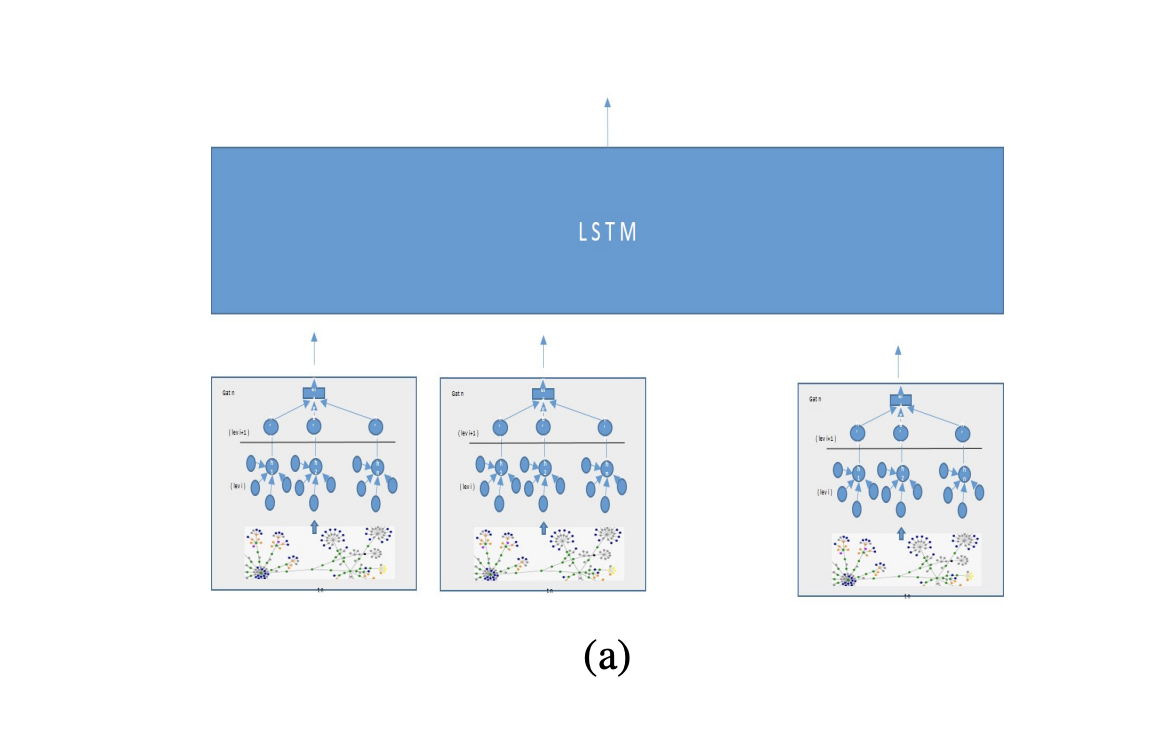
\includegraphics[width=0.7\linewidth]{3_step}
	\end{figure}
	\section*{Выводы}
	\addcontentsline{toc}{section}{Выводы}
	Таким образом, вышеописанные подходы для исследования ЭЭГ, являются актуальными и достаточно действенными. Однако, например, подход, основанный на ICA имеет проблемы с реплицируемостью, т.к. зачастую среди них применяются методы, актуальные только для тех данных, что были получены в рамках исследования.\\
	Однако, подходы, основанные на ICA имеют высокий уровень интерпретируемости, т.к. их можно выполнить и вручную, также, они располагают возможностью восстановления сигналов после разметки каждой из компонент на артефактную и нормальную.\\
	Подходы, основанные на автоэнкодерах имеют сложности с получением данных: т.к. автоэнкодеры обучаются на чистых и на зашумленных версиях тех же сигналов, то получение двух видов одной и той же ЭЭГ является сложной задачей и малоприменимо на практике. Однако, автоэнкодеры в перспективе могут показать наилучший результат, как они это делают в снижении шумов в изображениях.\\
	Были представлены ключевые метрики для сигналов, которые позволяют идентифицировать и получить информацию о том, что в них содержатся. Метрики разделены на временные, пространственные, спектральные и статистические. Оценка качества восстановленного сигнала проводится с помощью Signal-to-Noise ratio. Основной проблемой получения SNR является то, что часто получить точное соотношение невозможно, поэтому чаще лучше использовать классические метрики классификации.\\
	Графовые подходы оказались одними из наиболее удобно применимых на сырых данных и достаточно хорошо обобщаются для произвольных данных ЭЭГ, там лишь необходимо знать основные показатели сбора ЭЭГ. Однако, этот подход ещё не был применён для выявления артефактов в ЭЭГ и использован для классификации нормальных и нормальных ЭЭГ в целом.
	\chapter*{Построение подхода к решению поставленной задачи}
	\addcontentsline{toc}{chapter}{Построение подхода к решению поставленной задачи}
	\section*{Описание нейросетей, применяемых в работе}
	\addcontentsline{toc}{section}{Описание нейросетей, применяемых в работе}
	\subsection*{LSTM – сети долгой краткосрочной памяти}
	\addcontentsline{toc}{subsection}{LSTM – сети долгой краткосрочной памяти}
	Традиционные нейронные сети не обладают свойством сохранениях предыдущей информации, и в этом их главный недостаток. Представим, например, что мы хотим классифицировать события, происходящие в фильме. Непонятно, как традиционная нейронная сеть могла бы использовать рассуждения о предыдущих событиях фильма, чтобы получить информацию о последующих.
	
	Решить эту проблемы помогают рекуррентые нейронные сети (Recurrent Neural Networks, RNN). Это сети, содержащие обратные связи и позволяющие сохранять информацию.\\
	\begin{center} 
	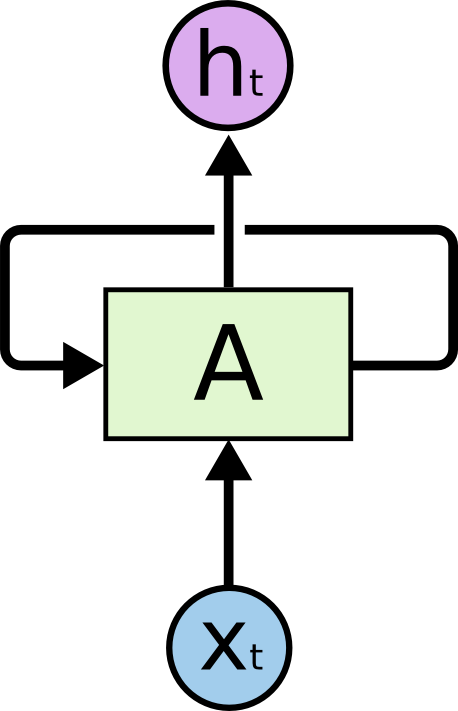
\includegraphics[scale=0.25]{neuron.png}\\
	\end{center}
	\textbf{Рекуррентные нейронные сети содержат обратные связи} На схеме выше фрагмент нейронной сети $A$  принимает входное значение $x_t$ и возвращает значение $h_t$. Наличие обратной связи позволяет передавать информацию от одного шага сети к другому. Рекуррентную сеть можно рассматривать, как несколько копий одной и той же сети, каждая из которых передает информацию последующей копии. Вот, что произойдет, если мы развернем обратную связь:
		\begin{center} 
		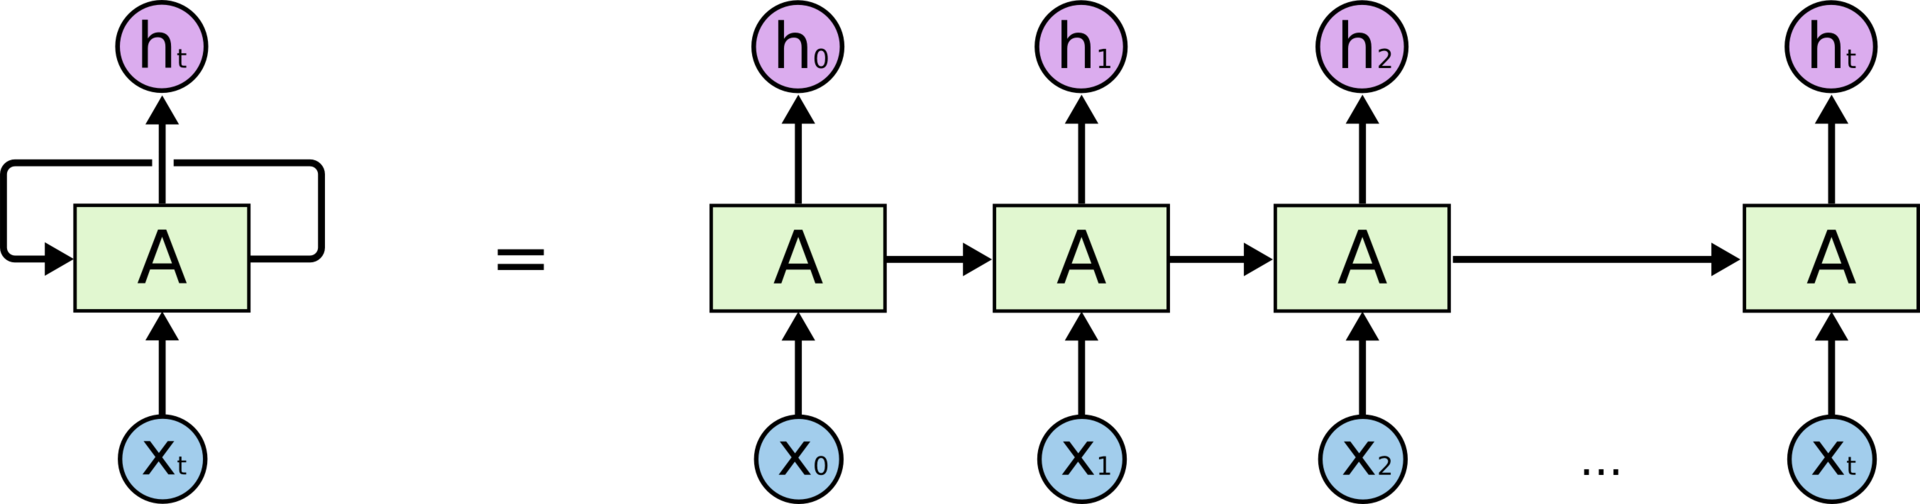
\includegraphics[scale=0.2]{rnn_returned.png}\\
	\end{center}
	То, что RNN напоминают цепочку, говорит о том, что они тесно связаны с последовательностями и списками. RNN – самая естественная архитектура нейронных сетей для работы с данными такого типа.
	Немалая роль в этих успехах принадлежит LSTM – необычной модификация рекуррентной нейронной сети, которая на многих задачах значительно превосходит стандартную версию.
	\subsubsection*{Проблема долговременных зависимостей}
	Одна из привлекательных идей RNN состоит в том, что они потенциально умеют связывать предыдущую информацию с текущей задачей, так, например, знания о предыдущем кадре видео могут помочь в понимании текущего кадра. Если бы RNN обладали такой способностью, они были бы чрезвычайно полезны. Но действительно ли RNN предоставляют нам такую возможность? Это зависит от некоторых обстоятельств.
	
	Иногда для выполнения текущей задачи нам необходима только недавняя информация. Рассмотрим, например, языковую модель, пытающуюся предсказать следующее слово на основании предыдущих. Если мы хотим предсказать последнее слово в предложении “облака плывут по небу”, нам не нужен более широкий контекст; в этом случае довольно очевидно, что последним словом будет “небу”. В этом случае, когда дистанция между актуальной информацией и местом, где она понадобилась, невелика, RNN могут обучиться использованию информации из прошлого.
		\begin{center} 
		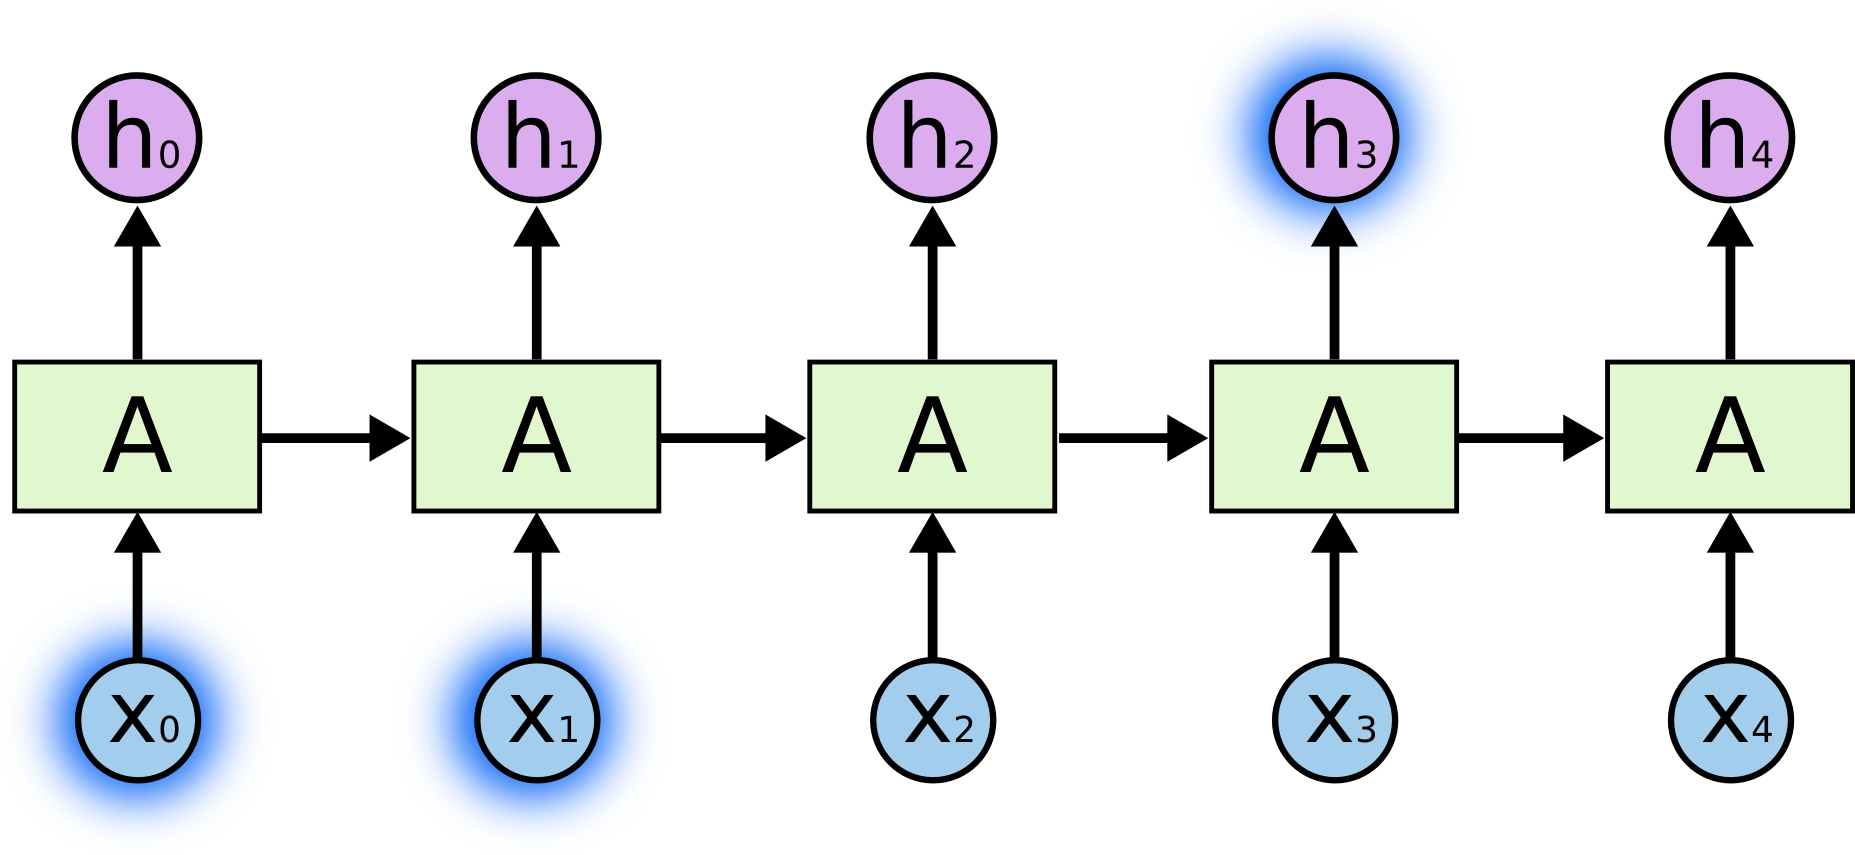
\includegraphics[scale=0.2]{activation_rnn.png}\\
	\end{center}
	Но бывают случаи, когда нам необходимо больше контекста. Допустим, мы хотим предсказать последнее слово в тексте “Я вырос во Франции… Я бегло говорю по-французски”. Ближайший контекст предполагает, что последним словом будет называние языка, но чтобы установить, какого именно языка, нам нужен контекст Франции из более отдаленного прошлого. Таким образом, разрыв между актуальной информацией и точкой ее применения может стать очень большим.
	
	К сожалению, по мере роста этого расстояния, RNN теряют способность связывать информацию.
	\begin{center} 
		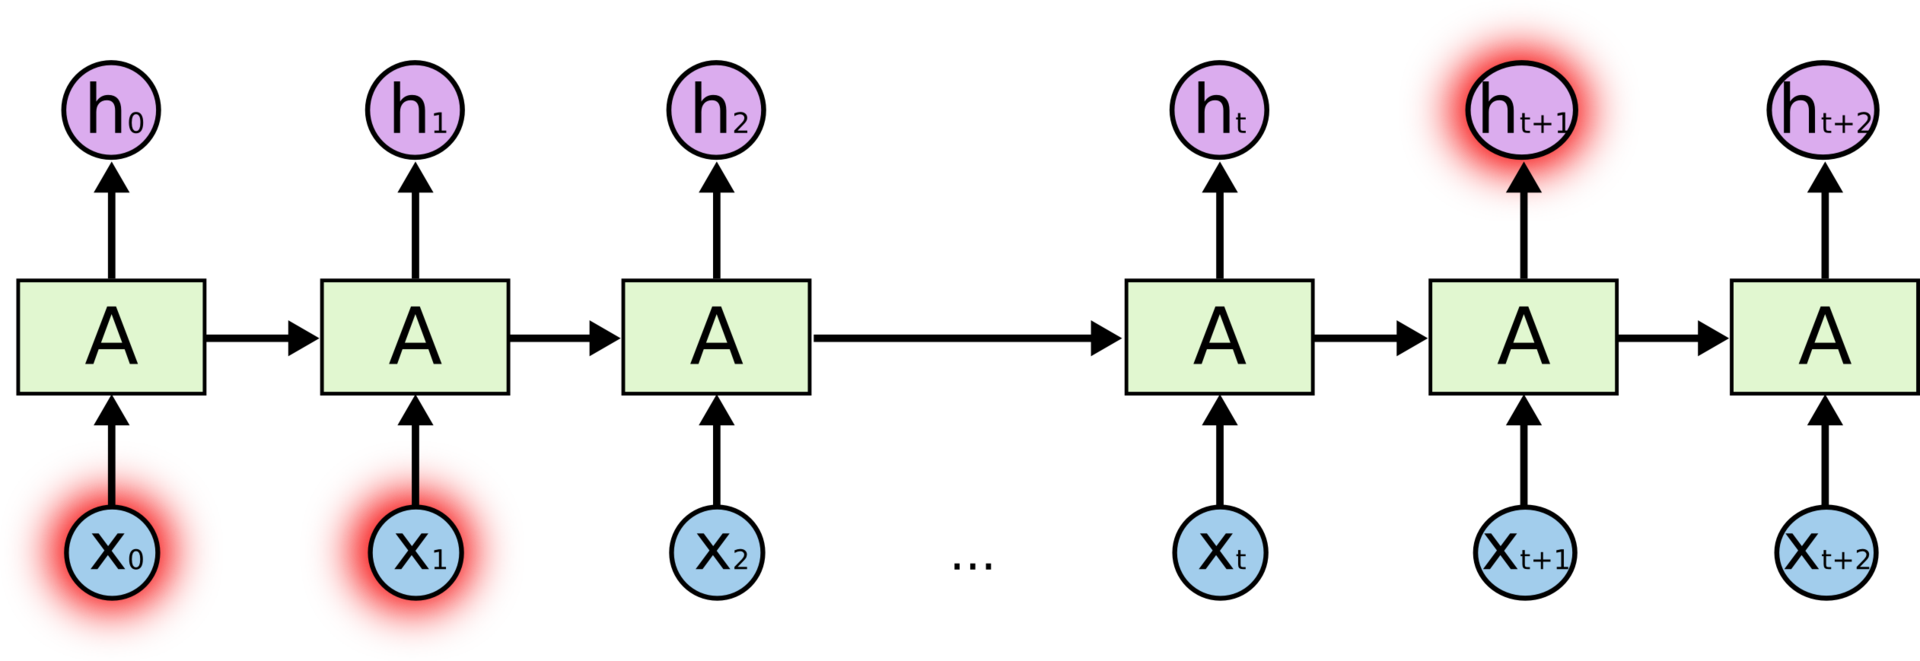
\includegraphics[scale=0.2]{problem_activation_rnn.png}\\
	\end{center}
	В теории проблемы с обработкой долговременных зависимостей у RNN быть не должно. Человек может аккуратно подбирать параметры сети для решения искусственные задачи такого типа. К сожалению, на практике обучить RNN этим параметрам кажется невозможным. Эту проблему подробно исследовали Иошуа Бенджио (Yoshua Bengio) с соавторами \cite{9}; они нашли неоспоримые причины, по которым это может быть сложно.
	\subsubsection*{Сети LSTM}
	Долгая краткосрочная память (Long short-term memory; LSTM) – особая разновидность архитектуры рекуррентных нейронных сетей, способная к обучению долговременным зависимостям. Они были представлены Зеппом Хохрайтер и Юргеном Шмидхубером (Jürgen Schmidhuber) в 1997 годy \cite{10}, а затем усовершенствованы и популярно изложены в работах многих других исследователей. Они прекрасно решают целый ряд разнообразных задач и в настоящее время широко используются.
	
	LSTM разработаны специально, чтобы избежать проблемы долговременной зависимости. Запоминание информации на долгие периоды времени – это их обычное поведение, а не что-то, чему они с трудом пытаются обучиться.
	
	Любая рекуррентная нейронная сеть имеет форму цепочки повторяющихся модулей нейронной сети. В обычной RNN структура одного такого модуля очень проста, например, он может представлять собой один слой с функцией активации tanh (гиперболический тангенс).
	\begin{center} 
		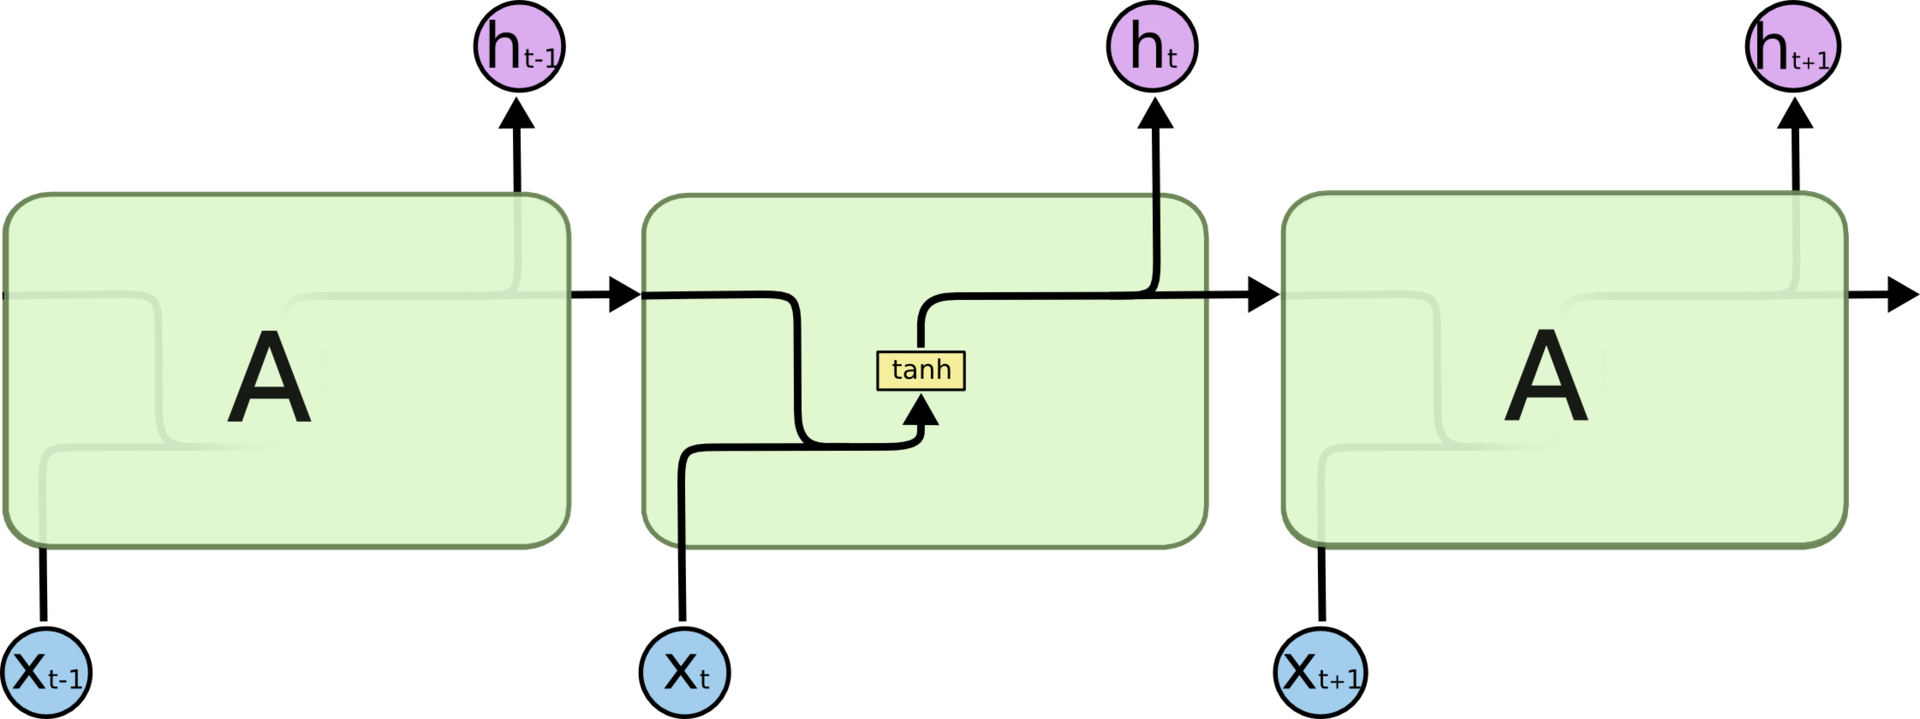
\includegraphics[scale=0.2]{tanh_act.png}\\
	\end{center}
	Повторяющийся модуль в стандартной RNN состоит из одного слоя.
	
	Структура LSTM также напоминает цепочку, но модули выглядят иначе. Вместо одного слоя нейронной сети они содержат целых четыре, и эти слои взаимодействуют особенным образом.
	\begin{center} 
		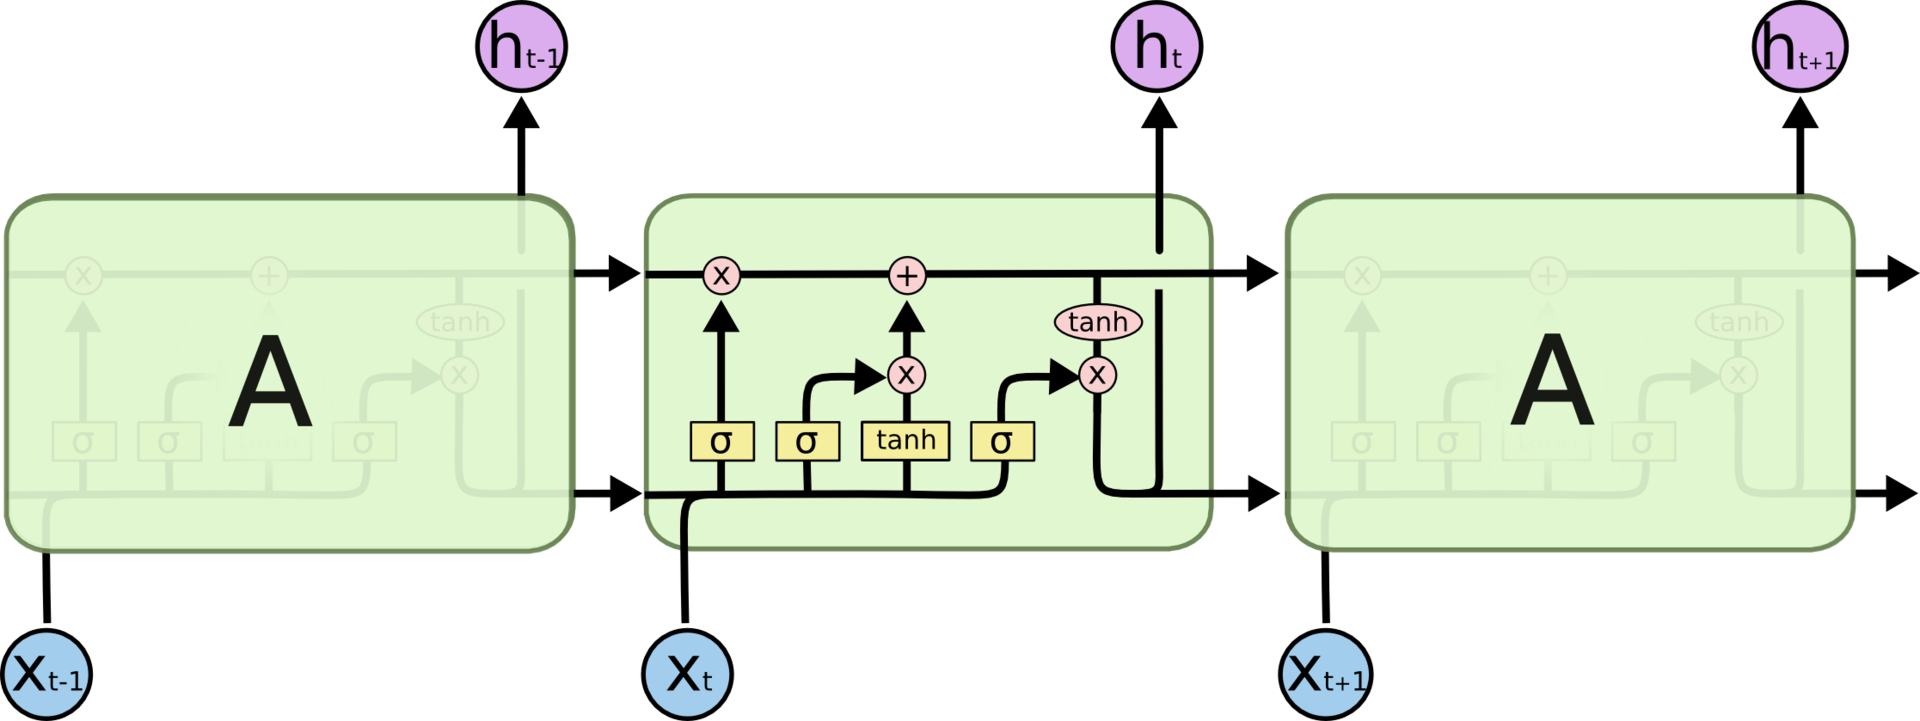
\includegraphics[scale=0.2]{lstm_act.png}\\
	\end{center}
	Повторяющийся модель в LSTM сети состоит из четырех взаимодействующих слоев.
	\begin{center} 
		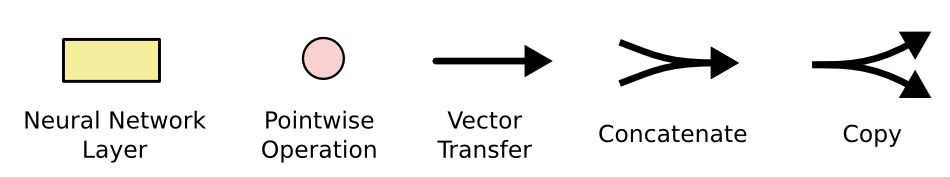
\includegraphics[scale=0.4]{layers_lstm.png}\\
	\end{center}
	На схеме выше каждая линия переносит целый вектор от выхода одного узла ко входу другого. Розовыми кружочками обозначены поточечные операции, такие, как сложение векторов, а желтые прямоугольники – это обученные слои нейронной сети. Сливающиеся линии означают объединение, а разветвляющиеся стрелки говорят о том, что данные копируются и копии уходят в разные компоненты сети.
	\subsection*{CNN - Сверточная нейронная сеть}
	\addcontentsline{toc}{subsection}{Сверточная нейронная сеть}
	Свёрточные нейронные сети основаны на операции свёртки:\\
	 \subsubsection*{Свертка}
	'''Свертка''' (англ. ''convolution'') - операция над парой матриц $A$ (размера $n_x\times n_y$) и $B$ (размера $m_x \times m_y$), результатом которой является матрица $C = A * B$ размера $(n_x-m_x+1)\times (n_y-m_y+1)$.
	Каждый элемент результата вычисляется как скалярное произведение матрицы $B$ и некоторой подматрицы $A$ такого же размера (подматрица определяется положением элемента в результате).
	То есть, $C_{i,j} = \sum_{u = 0}^{m_x-1}\sum_{v = 0}^{m_y - 1}A_{i+u,j+v}B_{u,v}$. На изображении справа можно видеть, как матрица $B$ «двигается» по матрице $A$, и в каждом положении считается скалярное произведение матрицы $B$ и той части матрицы $A$, на которую она сейчас наложена. Получившееся число записывается в соответствующий элемент результата.
	\subsubsection*{Структура сверточной нейронной сети}
	В сверточной нейронной сети выходы промежуточных слоев образуют матрицу (изображение) или набор матриц (несколько слоёв изображения). Так, например, на вход сверточной нейронной сети можно подавать три слоя изображения (R-, G-, B-каналы изображения). Основными видами слоев в сверточной нейронной сети являются сверточные слои (англ. ''convolutional layer''), пулинговые слои (англ. ''pooling layer'') и полносвязные слои (англ. ''fully-connected layer'').
	\subsubsection*{Сверточный слой}
	Сверточный слой нейронной сети представляет из себя применение операции свертки к выходам с предыдущего слоя, где веса ядра свертки являются обучаемыми параметрами. Еще один обучаемый вес используется в качестве константного сдвига (англ. ''bias''). При этом есть несколько важных деталей:
	\begin{itemize}
		\item  одном сверточном слое может быть несколько сверток. В этом случае для каждой свертки на выходе получится своё изображение. Например, если вход имел размерность $w\times h$, а в слое было $n$ сверток с ядром размерности $k_x\times k_y$, то выход будет иметь размерность $n\times(w - k_x + 1)\times(h - k_y + 1)$;
		\item Ядра свертки могут быть трёхмерными. Свертка трехмерного входа с трехмерным ядром происходит аналогично, просто скалярное произведение считается еще и по всем слоям изображения. Например, для усреднения информации о цветах исходного изображения, на первом слое можно использовать свертку размерности $3\times w \times h$. На выходе такого слоя будет уже одно изображение (вместо трёх);
		\item Можно заметить, что применение операции свертки уменьшает изображение. Также пиксели, которые находятся на границе изображения участвуют в меньшем количестве сверток, чем внутренние. В связи с этим в сверточных слоях используется дополнение изображения (англ. padding). Выходы с предыдущего слоя дополняются пикселями так, чтобы после свертки сохранился размер изображения. Такие свертки называют одинаковыми (англ. same convolution), а свертки без дополнения изображения называются правильными (англ. valid convolution).
		\item Еще одним параметром сверточного слоя является ''сдвиг'' (англ. ''stride''). Хоть обычно свертка применяется подряд для каждого пикселя, иногда используется сдвиг, отличный от единицы {{---}} скалярное произведение считается не со всеми возможными положениями ядра, а только с положениями, кратными некоторому сдвигу $s$. Тогда, если если вход имел размерность $w\times h$, а ядро свертки имело размерность $k_x\times k_y$ и использовался сдвиг $s$, то выход будет иметь размерность $\lfloor\frac{w - k_x}{s} + 1\rfloor\times\lfloor\frac{h - k_y}{s} + 1\rfloor$.
	\end{itemize}
	\begin{center} 
		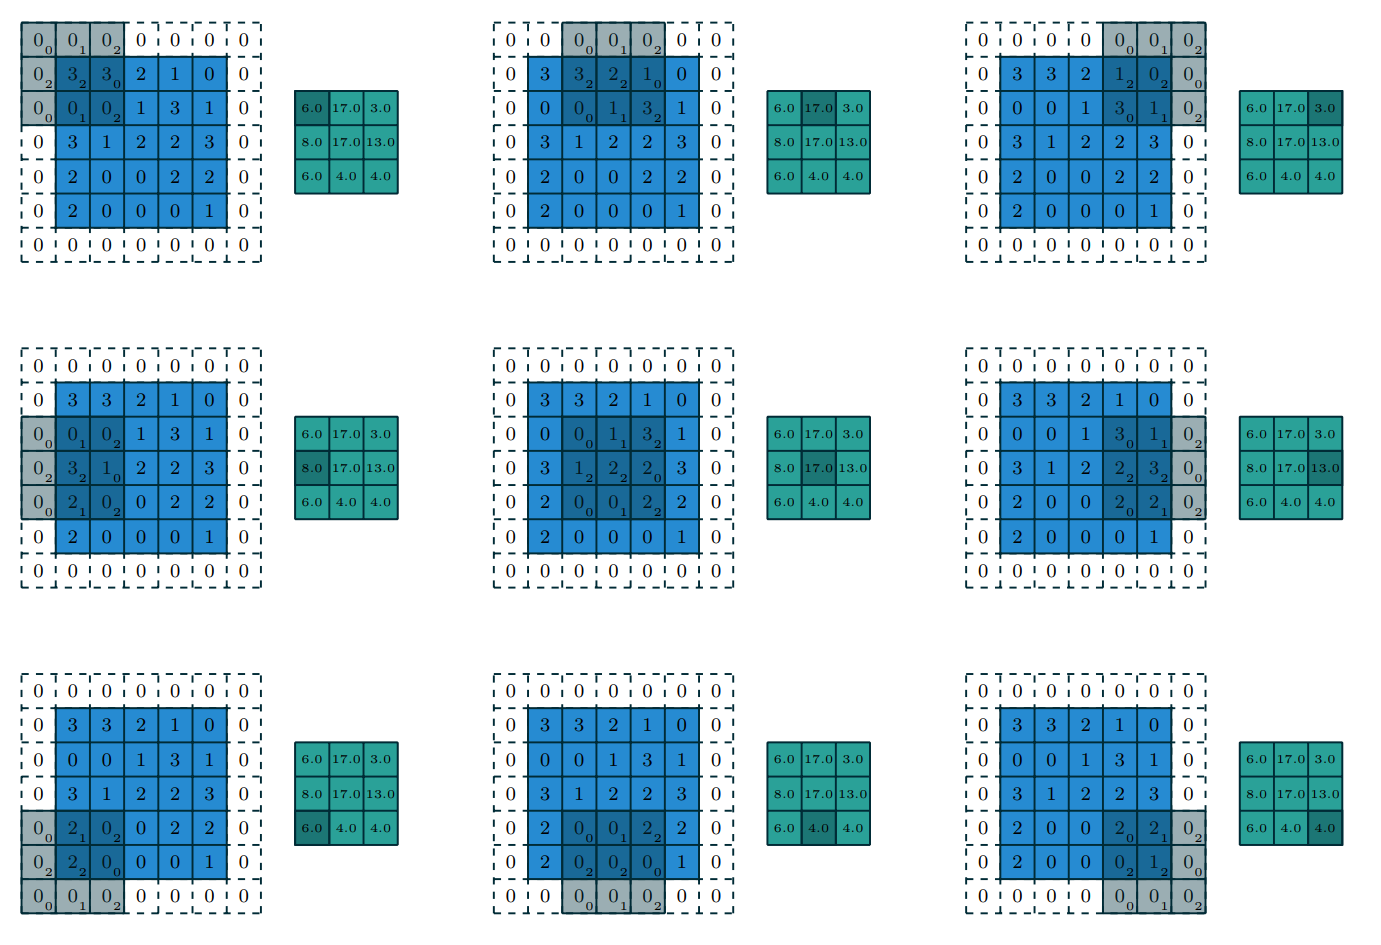
\includegraphics[scale=0.9]{Padding.png}\\
		Пример свертки двух матриц с дополнением нулями и сдвигом 2
	\end{center}
	\subsubsection*{Пулинговый слой}
	Пулинговый слой призван снижать размерность изображения. Исходное изображение делится на блоки размером $w\times h$ и для каждого блока вычисляется некоторая функция. Чаще всего используется функция максимума (англ. ''max pooling'') или (взвешенного) среднего (англ. ''(weighted) average pooling''). Обучаемых параметров у этого слоя нет. Основные цели пулингового слоя:
	\begin{itemize}
	\item  уменьшение изображения, чтобы последующие свертки оперировали над большей областью исходного изображения;
	\item увеличение инвариантности выхода сети по отношению к малому переносу входа;
	\item ускорение вычислений.
	\end{itemize}
	\begin{center} 
		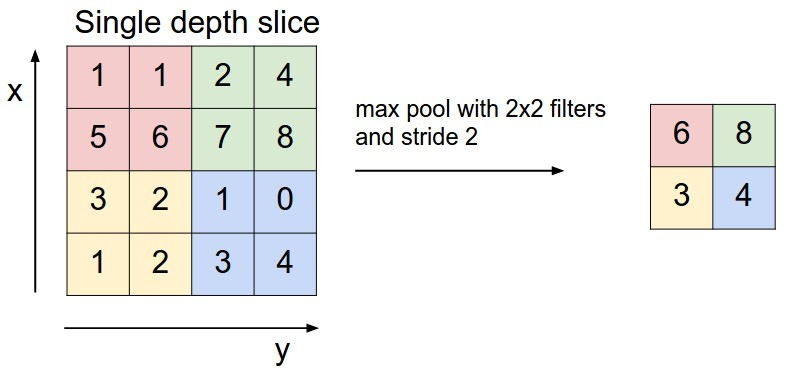
\includegraphics[scale=0.5]{Maxpool.jpeg}\\
		Пример операции пулинга с функцией максимума
	\end{center}
	\section*{Данные, на которых проводится исследование}
	\addcontentsline{toc}{section}{Данные, на которых проводится исследование}
	В работе применяется набор данных, собранных в Temple University: The TUH EEG Artifact Corpus. В нём представлены 259 сессий ЭЭГ от 213 пациентов. Данные представлены в edf формате (European Data Format) и в них размечены следующие артефакты:
	\begin{itemize}
		\item eyem: Движения глаз
		\item chew: Движение челюсти
		\item shiv: Дрожь
		\item elpp: Электростатические артефакты
		\item musc: Артефакты от сокращения мышц
		\item bckg: Фоновые
	\end{itemize}
	Артефакты размечены в отдельных файлах: Time-synchronous event (TSE) со следующим форматом\\
	
	0.0000 490.0000 bckg 1.0000\\
	
	Поля: Время начала в секундах, время окончания в секундах, тип и вероятность, равная единице\\
	Схема электродов следующая:\\
	 montage =  0, FP1-F7: EEG FP1-REF --  EEG F7-REF\\
	montage =  1, F7-T3:  EEG F7-REF  --  EEG T3-REF\\
	montage =  2, T3-T5:  EEG T3-REF  --  EEG T5-REF\\
	montage =  3, T5-O1:  EEG T5-REF  --  EEG O1-REF\\
	montage =  4, FP2-F8: EEG FP2-REF --  EEG F8-REF\\
	montage =  5, F8-T4 : EEG F8-REF  --  EEG T4-REF\\
	montage =  6, T4-T6:  EEG T4-REF  --  EEG T6-REF\\
	montage =  7, T6-O2:  EEG T6-REF  --  EEG O2-REF\\
	montage =  8, A1-T3:  EEG A1-REF  --  EEG T3-REF\\
	montage =  9, T3-C3:  EEG T3-REF  --  EEG C3-REF\\
	montage = 10, C3-CZ:  EEG C3-REF  --  EEG CZ-REF\\
	montage = 11, CZ-C4:  EEG CZ-REF  --  EEG C4-REF\\
	montage = 12, C4-T4:  EEG C4-REF  --  EEG T4-REF\\
	montage = 13, T4-A2:  EEG T4-REF  --  EEG A2-REF\\
	montage = 14, FP1-F3: EEG FP1-REF --  EEG F3-REF\\
	montage = 15, F3-C3:  EEG F3-REF  --  EEG C3-REF\\
	montage = 16, C3-P3:  EEG C3-REF  --  EEG P3-REF\\
	montage = 17, P3-O1:  EEG P3-REF  --  EEG O1-REF\\
	montage = 18, FP2-F4: EEG FP2-REF --  EEG F4-REF\\
	montage = 19, F4-C4:  EEG F4-REF  --  EEG C4-REF\\
	montage = 20, C4-P4:  EEG C4-REF  --  EEG P4-REF\\
	montage = 21, P4-O2:  EEG P4-REF  --  EEG O2-REF\\
	\begin{center} 
		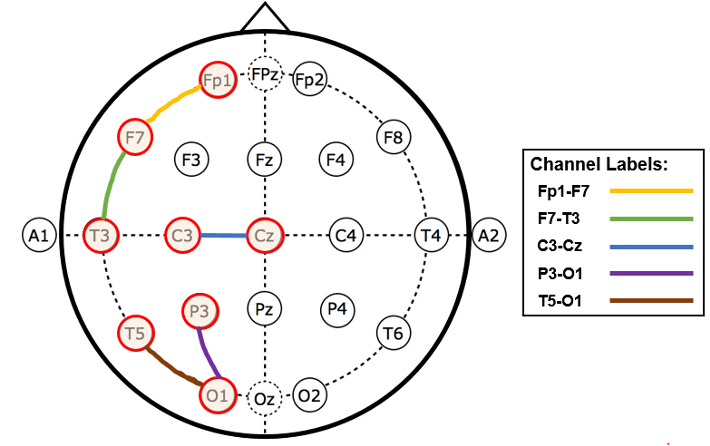
\includegraphics[scale=1]{montage_diploma.png}\\
		Схема расположения электродов
	\end{center}
	\section*{Постановка задачи классификации и метрики оценивания}
	\addcontentsline{toc}{section}{Постановка задачи классификации и метрики оценивания}
	\subsection*{Задача классификации}
	\addcontentsline{toc}{subsection}{Задача классификации}
	\subsubsection*{Постановка задачи}
	Пусть $X$ — множество описаний объектов, 
	$Y$ — множество номеров (или наименований) классов. 
	\\Существует неизвестная ''целевая зависимость'' — отображение
	$y^{*}\colon X\to Y$,
	значения которой известны только на объектах конечной выборки
	$X^m = \{(x_1,y_1),\dots,(x_m,y_m)\}$.
	Требуется построить алгоритм 
	$a\colon X\to Y$,
	способный классифицировать произвольный объект
	$x \in X$.\\
	Более общей считается вероятностная постановка задачи.\\
	Предполагается, что множество пар «объект, класс» 
	$X \times Y$
	является вероятностным пространством
	с неизвестной вероятностной мерой $\mathsf P$. 
	Имеется конечная выборка наблюдений
	$X^m = \{(x_1,y_1),\dots,(x_m,y_m)\}$, 
	сгенерированная согласно вероятностной мере $\mathsf P$. \\
	Требуется построить алгоритм 
	$a\colon X\to Y$,
	способный классифицировать произвольный объект
	$x \in X$.
	\subsubsection*{Классификация артефактов}
	В нашем случае, будет решаться задача бинарной классификации: необходимо разделить артефактные временные ряды, которые являются подмножеством временных рядов из данных ЭЭГ
	\subsubsection*{Метрики качества}
	Перед переходом к самим метрикам необходимо ввести важную концепцию для описания этих метрик в терминах ошибок классификации — confusion matrix (матрица ошибок).
	Допустим, что у нас есть два класса и алгоритм, предсказывающий принадлежность каждого объекта одному из классов, тогда матрица ошибок классификации будет выглядеть следующим образом:\\
		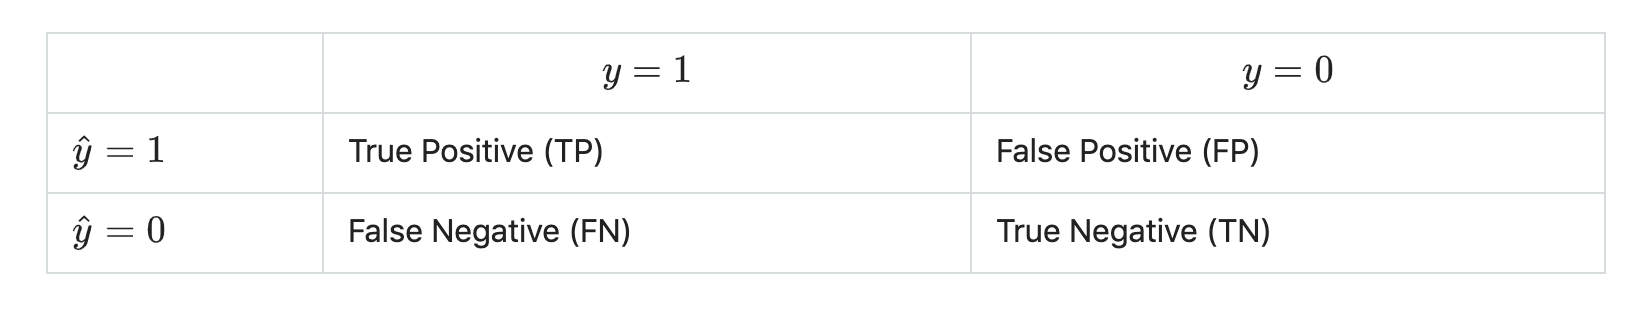
\includegraphics[scale=0.6]{matrix}\\
	Здесь $\hat{y}$ — это ответ алгоритма на объекте, а $y$  — истинная метка класса на этом объекте.
	Таким образом, ошибки классификации бывают двух видов: False Negative (FN) и False Positive (FP).\\
	Интуитивно понятной, очевидной и почти неиспользуемой метрикой является accuracy — доля правильных ответов алгоритма:
	$$
	\large accuracy = \frac{TP + TN}{TP + TN + FP + FN}
	$$
	Эта метрика бесполезна в задачах с неравными классами, и это легко показать на примере.\\
	Допустим, мы хотим оценить работу спам-фильтра почты. У нас есть 100 не-спам писем, 90 из которых наш классификатор определил верно (True Negative = 90, False Positive = 10), и 10 спам-писем, 5 из которых классификатор также определил верно (True Positive = 5, False Negative = 5).\\
	Тогда accuracy:\\
	$$
	\ accuracy = \frac{5 + 90}{5 + 90 + 10 + 5} = 86,4%
	$$
	Для оценки качества работы алгоритма на каждом из классов по отдельности введем метрики precision (точность) и recall (полнота).
	$$
	\large precision = \frac{TP}{TP + FP}
	$$
	$$
	\large recall = \frac{TP}{TP + FN}
	$$
	Precision можно интерпретировать как долю объектов, названных классификатором положительными и при этом действительно являющимися положительными, а recall показывает, какую долю объектов положительного класса из всех объектов положительного класса нашел алгоритм.\\
	Именно введение precision не позволяет нам записывать все объекты в один класс, так как в этом случае мы получаем рост уровня False Positive. Recall демонстрирует способность алгоритма обнаруживать данный класс вообще, а precision — способность отличать этот класс от других классов.\\
	Как мы отмечали ранее, ошибки классификации бывают двух видов: False Positive и False Negative. В статистике первый вид ошибок называют ошибкой I-го рода, а второй — ошибкой II-го рода. В нашей задаче по определению оттока абонентов, ошибкой первого рода будет принятие лояльного абонента за уходящего, так как наша нулевая гипотеза состоит в том, что никто из абонентов не уходит, а мы эту гипотезу отвергаем. Соответственно, ошибкой второго рода будет являться "пропуск" уходящего абонента и ошибочное принятие нулевой гипотезы.\\
	Precision и recall не зависят, в отличие от accuracy, от соотношения классов и потому применимы в условиях несбалансированных выборок.
	Часто в реальной практике стоит задача найти оптимальный (для заказчика) баланс между этими двумя метриками. Классическим примером является задача определения оттока клиентов.\\
	Очевидно, что мы не можем находить всех уходящих в отток клиентов и только их. Но, определив стратегию и ресурс для удержания клиентов, мы можем подобрать нужные пороги по precision и recall. Например, можно сосредоточиться на удержании только высокодоходных клиентов или тех, кто уйдет с большей вероятностью, так как мы ограничены в ресурсах колл-центра.\\
	Обычно при оптимизации гиперпараметров алгоритма (например, в случае перебора по сетке GridSearchCV ) используется одна метрика, улучшение которой мы и ожидаем увидеть на тестовой выборке.\\
	Существует несколько различных способов объединить precision и recall в агрегированный критерий качества. F-мера (в общем случае$\ F_\beta$ ) — среднее гармоническое precision и recall :
	$$
	\large \ F_\beta = (1 + \beta^2) \cdot \frac{precision \cdot recall}{(\beta^2 \cdot precision) + recall}
	$$
	$\beta$ в данном случае определяет вес точности в метрике, и при $\beta = 1$ это среднее гармоническое (с множителем 2, чтобы в случае precision = 1 и recall = 1 иметь $\ F_1 = 1$)
	F-мера достигает максимума при полноте и точности, равными единице, и близка к нулю, если один из аргументов близок к нулю.
	\section*{Предложенная архитектура решения и использования данных}
	\addcontentsline{toc}{section}{Предложенная архитектура решения и использования данных}
	\subsection*{Архитектура данных}
	\addcontentsline{toc}{section}{Архитектура данных}
	Представим данные в виде таймлайна графов, как показано в \cite{29}.\\
	Чтобы полноценно отобразить информацию, связанную со временем из ЭЭГ, применим подход, основанных на скользящих окнах, а именно:
	\begin{itemize}
		\item Многомерные данные разбиты на несколько пересекающихся окон по времени
		\item Каждый ряд из подвыборки используется, чтобы получить кросс-корреляционную матрицу, состоящую из значений корреляции Спирмена между каждым из каналов
	\end{itemize}
	Алгоритм работы с данными следующий:
		\begin{itemize}
		\item Сначала выбираются только те каналы, что представлены во всех датасетах - для этого реализован отдельный метод 
		\item Т.к. среди данных содержатся записи с различными частотами, необходимо свести их все к единой. Поэтому, реализован метод, выбирающий наименьшую частоту среди всех и выполняющий уменьшение частоты до заданной.
		\item Далее, применяется полосовой фильтр, чтобы снизить дисперсию сигналов. Также реализована версия без фильтра.
		\item Данные переформатируются в формат DataFrame для дальнейшего удобства
		\item Многомерные данные разбиты на несколько пересекающихся окон по времени
		\item Каждый ряд из подвыборки используется, чтобы получить кросс-корреляционную матрицу, состоящую из значений корреляции Спирмена между каждым из каналов
	\end{itemize}
	На выход после всех шагов, связанных с данными, подавалось 4494 фрагмента ЭЭГ с различными метками.
	\subsection*{Архитектура решения}
	\addcontentsline{toc}{section}{Архитектура решения}
	В качестве архитектуры, предлагается взять CNN с плотными (feed-forward) слоями, что позволяет, схоже с архитектурой, основанной на "внимании", получить для каждого окна эмбэддинг, который представляет соответствующий граф. Последовательность эмбеддингов может далее быть обработана, как вход из вложенных LSTM. Используемый оптимизатор: Adam - adaptive moment estimation \cite{45}\\
	В качестве второй архитектуры рассмотрим CNN без слоя LSTM, чтобы проверить улучшение или ухудшение качества в зависимости от наличия этого слоя. \\
	Устройство слоёв нейронной сети:
	\begin{enumerate}
		\item Слой Conv2D выполняет двумерную свертку между двумя последовательными слоями для каждой матрицы оцениваемой ЭЭГ.
		\item Слой MaxPooling2D концентрирует нейронные выходы из предыдущего слоя в отдельные нейроны следующего слоя, используя максимальное значение первого и таким образом уменьшая размерность после каждой операции.
		\item Слой Flatten схлопывает входные данные: например, если на вход поступает матрица, размерности [3,5], то на выход подаётся вектор размерности [15,]
		\item Слой Concat объединяет входы со слоя Flatten, на выход давая матрицу из векторов
		\item Слой LSTM 
		\item Dense - Нейроны в полносвязном слое связаны со всеми активационными нейронами предыдущего слоя, как это происходит в обычной нейронной сети. Активационная функция - softmax
	\end{enumerate}
	Схема сети c LSTM
	\\
	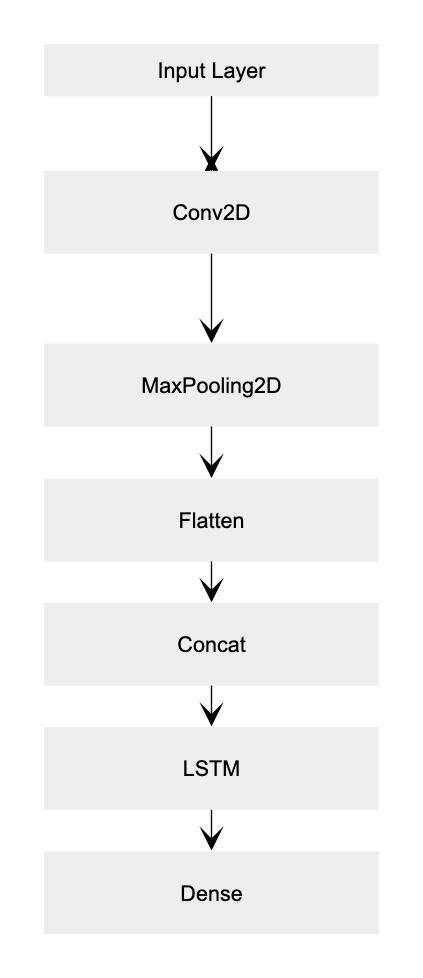
\includegraphics[scale=0.5]{layers.png}
	\\
	Схема сети без LSTM
	\\
	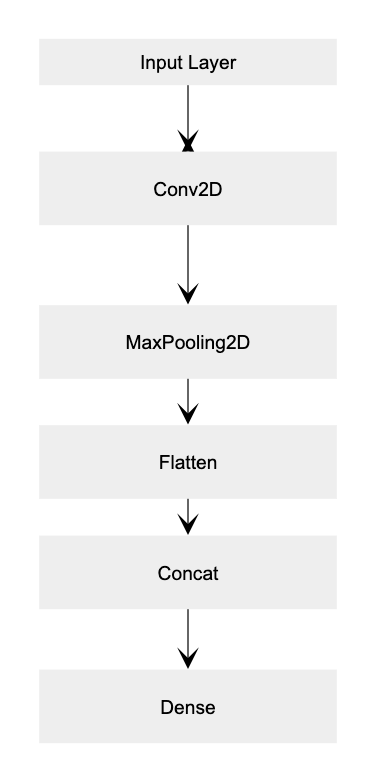
\includegraphics[scale=0.6]{layers_cnn.png}
	\\
	Также, для сравнения, предлагается использовать алгоритмы XGBoost и CatBoost, обучающиехся на тех же признаках, что и нейросети. 
	\section*{Выводы}
	\addcontentsline{toc}{section}{Выводы}
	В данной секции было предложено решение, основанное на нейросетях и классических алгоритмах машинного обучения. Также, была поставлена задача классификации, которая будет решаться, предложены метрики оценивания качества и целевая метрика. Целевой метрикой является f1-score, которая лучше всего подходит в этой задаче, т.к. она устойчива на несбалансированных классах.\\
	Был найден и описан датасет, в котором присутствуют размеченные артефакты 5 видов. Он был собран недавно и для него пока существует лишь один бенчмарк, в котором исследуются только алгоритмы классического машинного обучения и оптимизируются их параметры для получения наивысшего результата. Дальнейшая глава будет посвящена исследованию предложенного подхода и оценка его качества.
	\chapter*{Полученные результаты}
	\addcontentsline{toc}{chapter}{Полученные результаты}
	Обучение проводилось на локальной машине без GPU, технические спецификации следующие:\\
	\begin{itemize}
		\item Processor Name: Intel Core i5
		\item Processor Speed: 2.3 GHz
		\item Number of Processors: 1
		\item Total Number of Cores: 4
		\item L2 Cache (per Core): 256 KB
		\item L3 Cache: 6 MB
		\item Hyper-Threading Technology: Enabled
		\item Memory: 16 GB
	\end{itemize}
	Полученные результаты для различных вариаций после 5-фолдовой кросс-валидации модели можно увидеть в таблице ниже:\\
	\\
		\begin{tabular}{|l|l|l|l|}
			\hline
			Вид модели:               & f1\_score & accuracy \\ \hline
			CNN-LSTM bandpass фильтр + 16 окон & 0.67      & 0.71    \\ \hline
			CNN-LSTM Без фильтра + 4 окна      & 0.56      & 0.73    \\ \hline
			CNN-LSTM Bandpass фильтр + 8 окон + мультикласс      & 0.69      & 0.71   \\ \hline
			CNN-LSTM Bandpass фильтр + 8 окон + мультикласс + num\_epoch/2      & 0.7     & 0.71    \\ \hline
			CNN Bandpass фильтр + 8 окон + мультикласс   & 0.64     & 0.66    \\ \hline
			CNN + 8 окон + мультикласс   & 0.62     & 0.65    \\ \hline
			XGBoost + 8 окон + мультикласс   & 0.67     & 0.69    \\ \hline
			Catboost + 8 окон + мультикласс   & 0.62     & 0.64    \\ \hline
		\end{tabular}\\
	\\
	Таблица 1: Результаты алгоритмов на тестовом множестве\\
	\\
	Таким образом, видно, что применение частотного фильтра и увеличение количества окон положительно влияют на F-score, но снижает значение у accuracy, что в нашем случае не так сильно портит картину.\\
	Отдельно стоит отметить, что данные были изначально не самого высокого качества, т.к. были собраны в реальных условиях и применялись для диагностики пациентов. Лучший результат показала мультиклассовая классификация, со взвешенным f1-score. Таким образом, мультиклассовая классификация вместо бинарной показала себя лучше.
	Также, сеть показала способность переобучаться, т.к. представлено достаточно мало объектов различных классов. Это нейтрализуется уменьшением количества эпох.\\
	Рассмотрим confusion matrix для обоих видов сетей, которые использовались\\
	\begin{table}
		\begin{tabular}{|l|l|l|l| l| l|}
			\hline
			chew & elpp & eyem & musc & null & shiv  \\ \hline
			11   & 0    & 3    & 1    & 12   & 0     \\ \hline
			0    & 3    & 0    & 1    & 18   & 0     \\ \hline
			0    & 0    & 29   & 0    & 46   & 0     \\ \hline
			0    & 1    & 3    & 6    & 29   & 0     \\ \hline
			1    & 6    & 10   & 11   & 315  & 0     \\ \hline
			0    & 0    & 0    & 0    & 6    & 0    \\ \hline
		\end{tabular}\\
	Таблица 2: confusion matrix для CNN \\
	\end{table}	
	\\
		\begin{tabular}{|l|l|l|l| l| l|}
			\hline
				chew & elpp & eyem & musc & null & shiv   \\ \hline
				28&0&0&2&3&0 \\ \hline
				0&16&6&6&15&3 \\ \hline
				0&3&87&4&63&2 \\ \hline
				1&3&2&23&25&0 \\ \hline
				6&11&39&12&335&4 \\ \hline
				1&0&2&0&5&13 \\ \hline
		\end{tabular}\\
	Таблица 3: confusion matrix для CNN + LSTM \\
	\\
	\begin{tabular}{|l|l|l|l| l| l|}
		\hline
		chew & elpp & eyem & musc & null & shiv   \\ \hline
		 18 & 1 & 2 & 4 & 8 & 0  \\ \hline
		1 & 11 & 9 & 8 & 17 & 0  \\ \hline
		1 & 9 & 82 & 2 & 65 & 0  \\ \hline
		1 & 1 & 12 & 13 & 27 & 0  \\ \hline
		9 & 9 & 58 & 14 & 316 & 1  \\ \hline
		0 & 1 & 1 & 0 & 7 & 12  \\ \hline
	\end{tabular}\\
	Таблица 4: confusion matrix для Catboost \\
	\\
	\begin{tabular}{|l|l|l|l| l| l|}
		\hline
		chew & elpp & eyem & musc & null & shiv   \\ \hline
		23 & 0 & 0 & 0 & 10 & 0 \\ \hline
		0 & 5 & 4 & 1 & 36 & 0 \\ \hline
		0 & 0 & 85 & 1 & 73 & 0 \\ \hline
		0 & 1 & 6 & 20 & 27 & 0 \\ \hline
		7 & 5 & 39 & 1 & 355 & 0 \\ \hline
		0 & 1 & 1 & 0 & 8 & 11 \\ \hline
	\end{tabular}\\
	Таблица 5: confusion matrix для XGBoost \\
	Данные взяты из последних фолдов для кросс-валидации. Заметим, что большинству проставляются классы null, которые соответствуют данным без артефактов. Также, из-за малого количества данных класса shiv, он определяется очень плохо, эта проблема может быть решена увеличением выборки или же переходом к классификации секунд, а не периодов, как было сделано в \cite{35}. \\
	Также, наиболее частые классы артефактов вроде жевания и движения глаз выделяются лучше других, и шаг с LSTM улучшил результаты f1\_score.\\
	Если сравнить полученные результаты с классическими алгоритмами, которые являются стандартом в промышленности: CatBoost и XGBoost, то можно заметить, что эти алгоритмы в целом справляются с задачей хуже предложенного метода на основе нейросетей. Худшим среди всех оказался CatBoost, как по accuracy, так и по F1. Однако, интересно, что артефакты класса shiv, методы, основанные на бустинге, обнаруживают лучше нейросетевых.\\
	Модель на основе CNN+LSTM лучше остальных обнаруживает основные классы артефактов, поэтому её следует считать наилучшей среди всех остальных.\\
	Также, визуализируем функции потерь для нейросетей:\\
			\begin{center}
		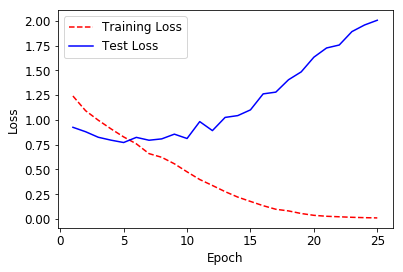
\includegraphics[scale=1]{loss_lstm.png}\\
		Функция потерь для CNN+LSTM на 25 эпохах на последнем фолде
	\end{center}
		\begin{center}
	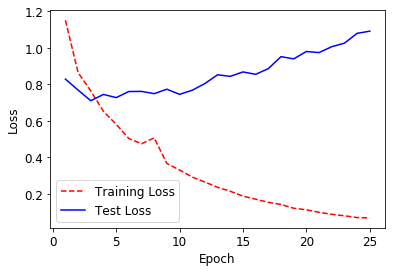
\includegraphics[scale=1]{cnn_loss.png}\\
	Функция потерь для CNN на 25 эпохах на последнем фолде
	\end{center}
	Из графиков выше, можно увидеть, что сети склонны к переобучению, что хорошо объясняется тем, что данных мало, поэтому можно легко пропустить какой-либо из видов артефактов при валидации. Это можно исправить двумя способами: уменьшить количество эпох, либо же увеличить количество данных, чтобы была возможность лучше увидеть все признаки. Также, заметно, что Loss у LSTM более резко идёт вверх на тесте, но плавнее снижается на обучении.
	В работе \cite{35} описаны результаты на том же датасете, но с классификацией не временных периодов, а секунд. Также, использовались другие признаки, была проведена оптимизация гиперпараметров. Сравним полученные результаты:\\
	\\
	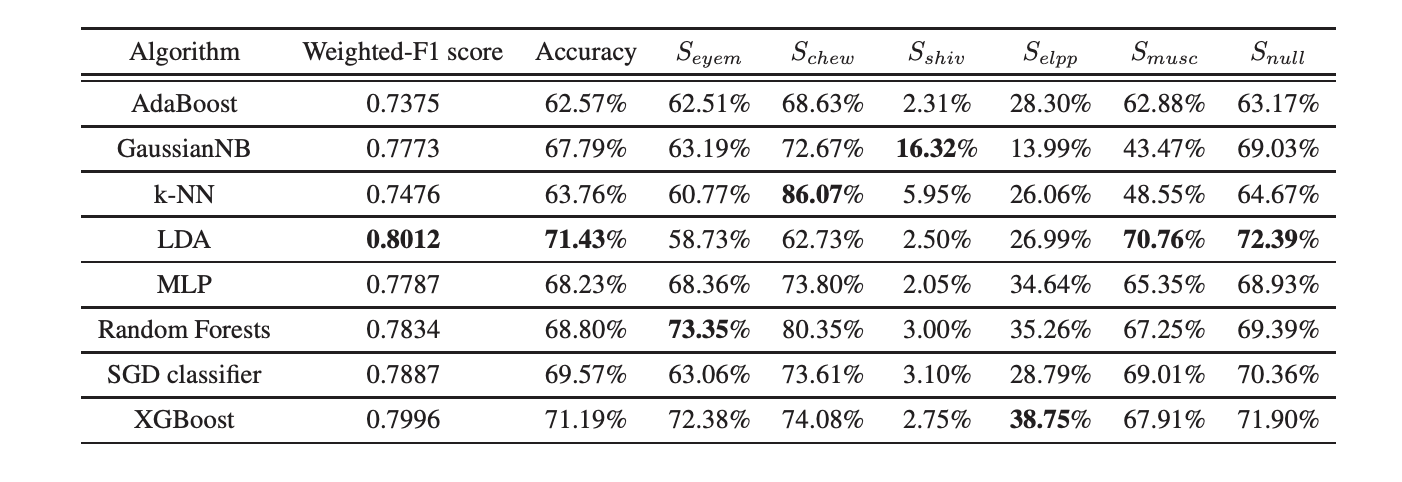
\includegraphics[scale=0.7]{results_other}
	\\
	Заметим, что общее значение accuracy в данной диссертации сравнимо с тем, что указано в \cite{35}. Повышенное значение f1\_score же обусловлено тем, что классифицировались секунды, а не более длинные периоды, таким образом было увеличено количество объектов различных классов и не применялись признаки, связанные со временем.Таким образом, полученные результаты дополняют изложенные бенчмарки, т.к. применяют нейросетевой подход, привязанный ко времени и графовой структуре.\\
	
	\chapter*{Заключение}
	\addcontentsline{toc}{chapter}{Заключение}
	В данной работе была рассмотрена задача классификации артефактов в сигналах ЭЭГ и особенности работы с такими данными в области их анализа. Был проведен подробный анализ существующих методов на основе «ручного» извлечения признаков и нейронных сетей глубокого обучения. \\
	Был получен доступ и исследован реальный набор данных из широкой выборки, что выделяет эту работу среди ранее описанных, т.к. данные, использовавшиеся в них были отчасти синтетическими, т.к. были получены не в полевых условиях  и не имели достаточно прозрачной процедуры их очистки\\
	Был реализован подход, основанный на нейронных сетях смешанной архитектуры, исследовавший графовую составляющую человеческого мозга.\\
	Полученные результаты могут использоваться в качестве дополнения бенчмарка для заданного набора данных (TUH EEG Dataset), что позволяет и далее улучшать предложенные в диссертации методы.
	\begin{thebibliography}{00}
			  \bibitem{1}
			 Gratton G., Coles M. G. H., Donchin E. A New Method for Off-Line Removal of Ocular Artifact. Electroencephalography and Clinical Neurophysiology, 1983, no. 55, pp. 468–484.
			 \bibitem{2}
			 Berg P., Scherg M. A Multiple Source Approach to the Correction of Eye Artifacts. Electroencephalography and Clinical Neurophysiology, 1994, no. 90, pp. 229–241.
			 \bibitem{3}
			 Bell A. J., Sejnowski T. J. An Information-Maximization Approach to Blind Separation and Blind Deconvolution. Neural Computation, 1995, no. 7, pp. 1129–1159.
			 \bibitem{4}
			 Lagerlund T. D., Sharbrough F. W., Busacker N. E. Spatial Filtering of Multichannel Electroencephalographic Recordings through Principal Component Analysis by Singular Value Decomposition. Journal of Clinical Neurophysiology, 1997, no. 1 (14), pp. 73–82.
			 \bibitem{5}
			 Jung T. P., Humphries C., Lee T. W., Makeig S., McKeown M. J., Iragui V., Sejnowski T. J. Extended ICA Removes Artifacts from Electroencephalographic Data.
			 Advances in Neural Information Processing Systems, 1998, no. 10, pp. 894–900.
			 \bibitem{6}
			 Gagnepain, J.-P \& Allouche, Laurent \& Toussaint, D \& Landre, Elisabeth. (2008). [From the analogic to the digital era: technical EEG progress for presurgical investigations of refractory partial epilepsies].. Neuro-Chirurgie. 54. 166-73. 
			 \bibitem{7}
			 Kobayashi K., James C. J., Nakahori T., Akiyama T., Gotman J. Isolation of Epileptiform Discharges from Unaveraged EEG by Independent Component Analysis. Journal of Clinical Neurophysiology, 1999, no. 10 (110), pp. 1755–1763.
			 \bibitem{8}
			 Delorme A., Makeig S., Sejnowski T. Automatic Artifact Rejection for EEG Data using High-Order Statistics and Independent Component Analysis. Proc. of the Third Intern. ICA Conf., San Diego, USA, December 2001, pp. 9–12.
			 \bibitem{9}
			 Y. Bengio, P. Simard and P. Frasconi, "Learning long-term dependencies with gradient descent is difficult," in IEEE Transactions on Neural Networks, vol. 5, no. 2, pp. 157-166, March 1994, doi: 10.1109/72.279181.
			 \bibitem{10}
			 Hochreiter, Sepp \& Schmidhuber, Jürgen. (1997). Long Short-term Memory. Neural computation. 9. 1735-80. 10.1162/neco.1997.9.8.1735. 
			 \bibitem{11}
			Frasconi, P., Gori, M., and Sperduti, A. (1998). A general
			framework for adaptive processing of data structures.
			IEEE transactions on Neural Networks, 9(5):768–
			786.
			\bibitem{12}
			Gers, F. A., Schmidhuber, J., and Cummins, F. (1999).
			Learning to forget: Continual prediction with lstm.
			Gori, M., Monfardini, G., and Scarselli, F. (2005). A new
			model for learning in graph domains. In Proceedings.
			2005 IEEE International Joint Conference on Neural
			Networks, 2005., volume 2, pages 729–734. IEEE.
			\bibitem{13}
			Goyal, P. and Ferrara, E. (2018). Graph embedding techniques, applications, and performance: A survey.
			Knowledge-Based Systems, 151:78–94.
			Grattarola, D. (2019). danielegrattarola/spektral.
			\bibitem{14}
			Lee, J. B., Rossi, R. A., Kim, S., Ahmed, N. K., and Koh, E.
			(2018). Attention models in graphs: A survey. arXiv
			preprint arXiv:1807.07984.
			\bibitem{15}
			Lopez, S., Suarez, G., Jungreis, D., Obeid, I., and Picone,
			J. (2015). Automated identification of abnormal adult
			eegs.
			\bibitem{16}
			Obeid, I. and Picone, J. (2016). The temple university
			hospital eeg data corpus. Frontiers in neuroscience,
			10:196.
			\bibitem{17}
			Rubinov, M. and Sporns, O. (2010). Complex network measures of brain connectivity: uses and interpretations.
			Neuroimage, 52(3):1059–1069.
			\bibitem{18}
			Scarselli, F., Gori, M., Tsoi, A. C., Hagenbuchner, M.,
			and Monfardini, G. (2008). The graph neural network model. IEEE Transactions on Neural Networks,
			20(1):61–80.
			\bibitem{19}
			Schirrmeister, R. T., Gemein, L., Eggensperger, K., Hutter,
			F., and Ball, T. (2017). Deep learning with convolutional neural networks for decoding and visualization
			of eeg pathology.
			\bibitem{20}
			Shih, C.-T., Sporns, O., Yuan, S.-L., Su, T.-S., Lin, Y.-J.,
			Chuang, C.-C., Wang, T.-Y., Lo, C.-C., Greenspan,
			R. J., and Chiang, A.-S. (2015). Connectomics-based
			analysis of information flow in the drosophila brain.
			Current Biology, 25(10):1249–1258.
			\bibitem{21}
			Towlson, E. K., Vertes, P. E., Ahnert, S. E., Schafer, W. R., 
			and Bullmore, E. T. (2013). The rich club of the c. elegans neuronal connectome. Journal of Neuroscience,
			33(15):6380–6387.
			\bibitem{22}
			van den Heuvel, M. P., Kahn, R. S., Goni, J., and Sporns, O. ˜
			(2012). High-cost, high-capacity backbone for global
			brain communication. Proceedings of the National
			Academy of Sciences, 109(28):11372–11377.
			\bibitem{23}
			Varela, F., Lachaux, J.-P., Rodriguez, E., and Martinerie,
			J. (2001). The brainweb: phase synchronization and
			large-scale integration. Nature reviews neuroscience,
			2(4):229.
			\bibitem{24}
			Velickovic, P., Cucurull, G., Casanova, A., Romero, A., Lio,
			P., and Bengio, Y. (2017). Graph attention networks.
			arXiv preprint arXiv:1710.10903.
			\bibitem{25}
			Ozal Yıldırım, Baloglu, U. B., and Acharya, U. R. (2017). 
			A deep convolutional neural network model for automated identification of abnormal eeg signals.
			\bibitem{26 }
			Sperduti, A. and Starita, A. (1997). Supervised neural networks for the classification of structures. IEEE Transactions on Neural Networks, 8(3):714–735.
			\bibitem{27}
			Stone DB, Gabriella T, Patrique F, Jens H, Silvia C. Automatic Removal of Physiological Artifacts in EEG: The Optimized Fingerprint Method for Sports Science Applications. Frontiers in Human Neuroscience . 2018;12:96.
			\bibitem{28}
			Raduntz T, Scouten J, Hochmuth O, Meffert B. EEG artifact elimination by extraction of ICA-component features
			using image processing algorithms. Journal of Neuroscience Methods. 2015;243:84-93.
			\bibitem{29}
			Zoppis, I.; Zanga, Alessio; Manzoni, S.; Cisotto, G.; Morreale, A.; Stella, F. and Mauri, G. (2020). An Attention-based Architecture for EEG Classification.In Proceedings of the 13th International Joint Conference on Biomedical Engineering Systems and Technologies - Volume 4: BIOSIGNALS, ISBN 978-989-758-398-8, pages 214-219. DOI: 10.5220/0008953502140219
			\bibitem{30}
			Tamburro, Gabriella \& Fiedler, Patrique \& Stone, David \& Haueisen, Jens \& Comani, Silvia. (2018). A new ICA-based fingerprint method for the automatic removal of physiological artifacts from EEG recordings. PeerJ. 6. 10.7717/peerj.4380. 
			\bibitem{31}
			https://emedicine.medscape.com/article/1140247-overview
			\bibitem{32}
			Pion-Tonachini, Luca, Ken Kreutz-Delgado, and Scott Makeig. “ICLabel: An Automated Electroencephalographic Independent Component Classifier, Dataset, and Website.” NeuroImage 198 (2019): 181–197. Crossref. Web.
			\bibitem{33}Dowding, Irene \& Haufe, Stefan \& Tangermann, Michael. (2011). Automatic Classification of Artifactual ICA-Components for Artifact Removal in EEG Signals. Behavioral and brain functions : BBF. 7. 30. 10.1186/1744-9081-7-30. 
			\bibitem{34} "DEAP: A Database for Emotion Analysis using Physiological Signals (PDF)", S. Koelstra, C. Muehl, M. Soleymani, J.-S. Lee, A. Yazdani, T. Ebrahimi, T. Pun, A. Nijholt, I. Patras, IEEE Transaction on Affective Computing, Special Issue on Naturalistic Affect Resources for System Building and Evaluation, in press
			\bibitem{35} Roy, Subhrajit. (2019). Machine Learning for removing EEG artifacts: Setting the benchmark. 
			\bibitem{36}
			Yannick Roy and Hubert Banville and Isabela Albuquerque and Alexandre Gramfort and Tiago H. Falk and Jocelyn Faubert, Deep learning-based electroencephalography analysis: a systematic review, 2019
			\bibitem{37}
			Bhattacharjee, Snehashish \& Ghatak, Sujata \& Dutta, Soumi \& Chatterjee, Biswajoy \& Gupta, Mousumi. (2019). A Survey on Comparison Analysis Between EEG Signal and MRI for Brain Stroke Detection: Proceedings of IEMIS 2018, Volume 3. 10.1007/978-981-13-1501-5\_32. 
			\bibitem{38}
			https://imotions.com/hardware/abm-b-alert-x10/
			\bibitem{39}
			Raboel, Peter \& Bartek, J \& Andresen, M \& Bellander, Bo-Michael \& Romner, B. (2012). Intracranial Pressure Monitoring: Invasive versus Non-Invasive Methods—A Review. Critical care research and practice. 2012. 950393. 10.1155/2012/950393.
			\bibitem{40}
			Acharya, Jayant \& Acharya, Vinita. (2019). Overview of EEG Montages and Principles of Localization. Journal of clinical neurophysiology : official publication of the American Electroencephalographic Society. 36. 325-329. 10.1097/WNP.0000000000000538.  
			\bibitem{41}
			Kalra, Anubha \& Anand, Gautam \& Lowe, Andrew. (2020). Interpreting Electroencephalogram (EEG) – An Introductory Review of Assessment and Measurement Procedures. Modern Applied Science. 14. 47. 10.5539/mas.v14n6p47. 
			\bibitem{42}
			Niedermeyer, E. (1997). Alpha rhythms as physiological and abnormal phenomena. Int. J. Psychophysiol. Off. J.
			Int. Organ. Psychophysiol, 26, 31–49. https://doi.org/10.1016/s0167-8760(97)00754-x 
			\bibitem{43}
			Julie Onton, Marissa Westerfield, Jeanne Townsend, Scott Makeig,
			Imaging human EEG dynamics using independent component analysis,
			Neuroscience \& Biobehavioral Reviews,
			Volume 30, Issue 6,
			2006,
			Pages 808-822,
			ISSN 0149-7634,
			https://doi.org/10.1016/j.neubiorev.2006.06.007.
			\bibitem{44}
			Tatum, William \& Dworetzky, Barbara \& Schomer, Donald. (2011). Artifact and Recording Concepts in EEG. Journal of clinical neurophysiology : official publication of the American Electroencephalographic Society. 28. 252-63. 10.1097/WNP.0b013e31821c3c93. 
			\bibitem{45}
			Kingma, Diederik \& Ba, Jimmy. (2014). Adam: A Method for Stochastic Optimization. International Conference on Learning Representations. 
	\end{thebibliography} 
\end{document}